\documentclass[a4paper,twoside,10pt]{report}
\usepackage[english]{babel}
\usepackage[utf8]{inputenc}
\usepackage{graphicx}
\usepackage{url}
\usepackage{pdfpages}
\usepackage[export]{adjustbox}
\usepackage{indentfirst}
% pdflatex

% redefinição das margens das páginas
\setlength{\textheight}{24.00cm}
\setlength{\textwidth}{15.50cm}
\setlength{\topmargin}{0.35cm}
\setlength{\headheight}{0cm}
\setlength{\headsep}{0cm}
\setlength{\oddsidemargin}{0.25cm}
\setlength{\evensidemargin}{0.25cm}
\setlength{\parskip}{1em}

\begin{document}

\begin{figure}[t]
\resizebox{60mm}{!}{
\includegraphics[left]{logoISEL.png}}
\end{figure}

\title{\huge\textbf{Lean Dashboard}}

\author{
\begin{tabular}{c}
José Pedro Jesus, n.º 44805\\
Hugo Manuel Jacinto Pinheiro, n.º 44886\\
Tomás Simão Mendes dos Santos, n.º 45363\\
\end{tabular}
}

\date{
\begin{tabular}{ll}
 {\textbf{Supervisors:}} & João Pereira, e-mail: joao.pereira@inetum.world, Inetum \\
         & Filipe Freitas, e-mail: ffreitas@cc.isel.ipl.pt\\
\end{tabular}\\
\vspace{80mm}
\textbf{June 14th 2021}}

\maketitle

\title{\huge\textbf{Abstract}}

The amount of information necessary to develop an application nowadays is a lot to keep track of. Suppose you're a project manager and you want to keep track of the information of your project as well as show it to your team, but it is scattered across different platforms.

Data ranging from test results to the current sprints can all be puzzle pieces of a much bigger picture and accessing the various platforms only to view this information can be tiring and complicated. This project's goal is to simplify a team's life, by developing an application that allows a project manager to control and show the team members the necessary information for their project.

This application will make use of a single page application, a web server(Web API), as well as a no-SQL database, and an ETL procedure used to extract and transform the information from the various data sources.


\textbf{Keywords:} Information Aggregation, ETL, Project Managing, Project Information, Team Management, Single Page Application, Web API, no-SQL Database


\newpage
\tableofcontents{}
\newpage

\chapter{Introduction}

Nowadays, within a company, it is even more important to have an organized and cooperative team with knowledge of all the steps and goals that need to be worked on for the various projects they are currently participating in.
Each member of the team must keep track of high amounts of information and since it is not uncommon that when working on a project a couple of platforms are used to keep track and share work done by the various members, useful information can be scattered on a vast amount of platforms, and sometimes even inside a single platform.
The information relative to a project can be obtained from different sources and it is all aggregated in one place, readily available to be displayed to a work team to better guide a certain project's development.

The Lean Dashboard Project was developed to help the company's workers keeping track of all the possible tasks for their projects, gathering all the information needed for the various activities from the many sources that are necessary, presenting it on an easy to read and reactive web application.
The project at hands was developed in partnership with Inetum\cite{INETUM} and centred around the development of a responsive web application capable of running on a multitude of devices, ranging from smartphones to desktop computers to large screens such as TVs. This web application displays to a work team of a company all the information regarding various projects being worked on. 
The information being displayed shows the team what needs to be addressed in the project at hands, such as milestones, bugs, and current errors in the project.

The project required the development of 3 principal components: an ETL procedure, a web API, and a client application. This report will explain these 3 components in more depth further on.
The first two were developed using the Node.JS programming language while the client application was developed using the React library.

\section{Report Organization}
In this report, we explain the implemented solution to the problem at hand, as well as provide a more in-depth analysis of the architecture and technology choices. The organization of the report is based on the temporal order that we made throughout the project.

In the Functionalities chapter, we will expose the features that were implemented for the project's application. Additionally, we also showcase a couple of aspects regarding planning and research.

Next up, in the Architecture chapter, we will discuss aspects such as the implementation of the software being developed, decisions made by us and how certain problems were solved.

Furthermore, we dedicate a chapter to the research done regarding User Experience for our application where we display some of the steps, we took in preparing our client application in terms of User Experience.

On the Client Application chapter, we explain the reason for the chosen development platform, how the client application works and display some of the web pages.  

In the Deployment chapter, we explain the choices made for the deployment platform and how it was made. Finally, in the Conclusion chapter, we expose the learned lessons and future work for forthcoming versions.

\chapter{Functionalities}

The functionalities chapter is destined to list and describe the functionalities that the application provides the user with.

The solution is a responsive mobile-first web application that allows the user to consult and aggregate the information of various platforms. Inside a project, a manager is to be able to add various dashboards that will then have the desired widgets. The widgets are the structures that hold and show the desired information regarding issues, tests, and sprints from platforms such as Jira\cite{JIRA}, Squash\cite{SQUASH} and Azure\cite{AZURE}. A manager will then be able to add various users to its project so that those users can consult all the dashboards with the relevant information in each widget.

These are the features implemented within the application:
 
\begin{itemize}
   \item Retrieving the data from the multiple APIs. We can access three supported APIs to obtain the relevant information, these being Jira, Squash and Azure.
   
   \item Authentication of local users using the Authization Module. With the help of the module, we can create and edit users, log in, and log out users of local accounts.
   
   \item In addition to users, we also support roles for the given users: Superuser, Manager, and Collaborator.
   
   \item Back-office functionality. With this, managers can do actions such as add new members to a project, remove current project members as well as give certain users roles.

   \item Creating new projects. Authorized users can add new projects to the platform and manage them.

   \item Creating various Dashboards inside an existing project. After creating a project, it is also possible to include new dashboards in said project.

   \item Transforming the retrieved data in a widget format.

   \item Creating a widget and adding it to an existing dashboard with the use of existing templates, that aid the user by showing them the type of existing widgets.

   \item Automatically updating widgets with the use of a scheduler. Users can set a period to refresh existing widgets, making sure the most up-to-date information is being displayed. The process and technology chosen for the scheduler are explained in the back-end portion of this report.

   \item Setting the credentials for all the platforms. When creating a widget, a user can set up the desired credentials, to choose the data source for a specific widget.

   \item Front-end client application based on React technology.
   
   \item Presentation mode for large screens. Dashboards are presented in slideshow format.

   \item Multi-language support for the client application.

\end{itemize}

Throughout this report, we will explain how we implement these features.

\chapter{Architecture}
This chapter is dedicated to cover topics like the software's architecture, the data model, and the principles under which the application was developed. 

It contains information on how the application works and how its various modules and components interact with each other, as well as the structure of the necessary information being stored in the database and the application's authentication and authorization flow.
\section{Architecture Principles and Components}
The software solution in the Lean Dashboard is divided into three main components: the ETL\cite{ETLPROC}, the Lean Dashboard Server, and the client application.
 
The ETL component, which stands for Extract, Transform and Load, is responsible for obtaining the information from the various APIs and then transforming it to the desired format, widgets, and then proceeding to store them in a database. Both the topics of widgets and the storage solution being used are addressed in this report in the Data model.
 
With the use of the ETL procedure in our application, we bring a couple of advantages to the way we interact with the data being displayed. Since having near-real-time information is enough, with the Extract component we can avoid making high amounts of requests to the various APIs and avoiding overload them.
 
Additionally, by adapting the extracted information (the Transform component) we can have a format of data that closely resembles the type and aspect of details we are trying to show to the user in each widget (we will also showcase the aspect of a widget in our application). Finally, with the information transformed to the desired format, when can then use a No-SQL database to store it and later use that information to display to the users 
 
The Lean Dashboard server ends up serving as a gatherer of information. Inside this server, we have all the various projects, created by users, and each one will have its dashboards. Dashboards will be used to group the various widgets, and the user is the one to choose which dashboards will contain which widgets (these being the same widgets that we're created by the Extract, Transform, and Load procedure).
 
Lastly, we have the client application. The client application is responsible for showing the user all its projects. Users (if they are given these permissions) will be able to consult but also edit projects and dashboards. The main goal will be checking on the widgets inside a certain dashboard since those are the objects that contain the information being retrieved and transformed by the ETL.

\section{Software Architecture}
\begin{figure}[h!]
\center
  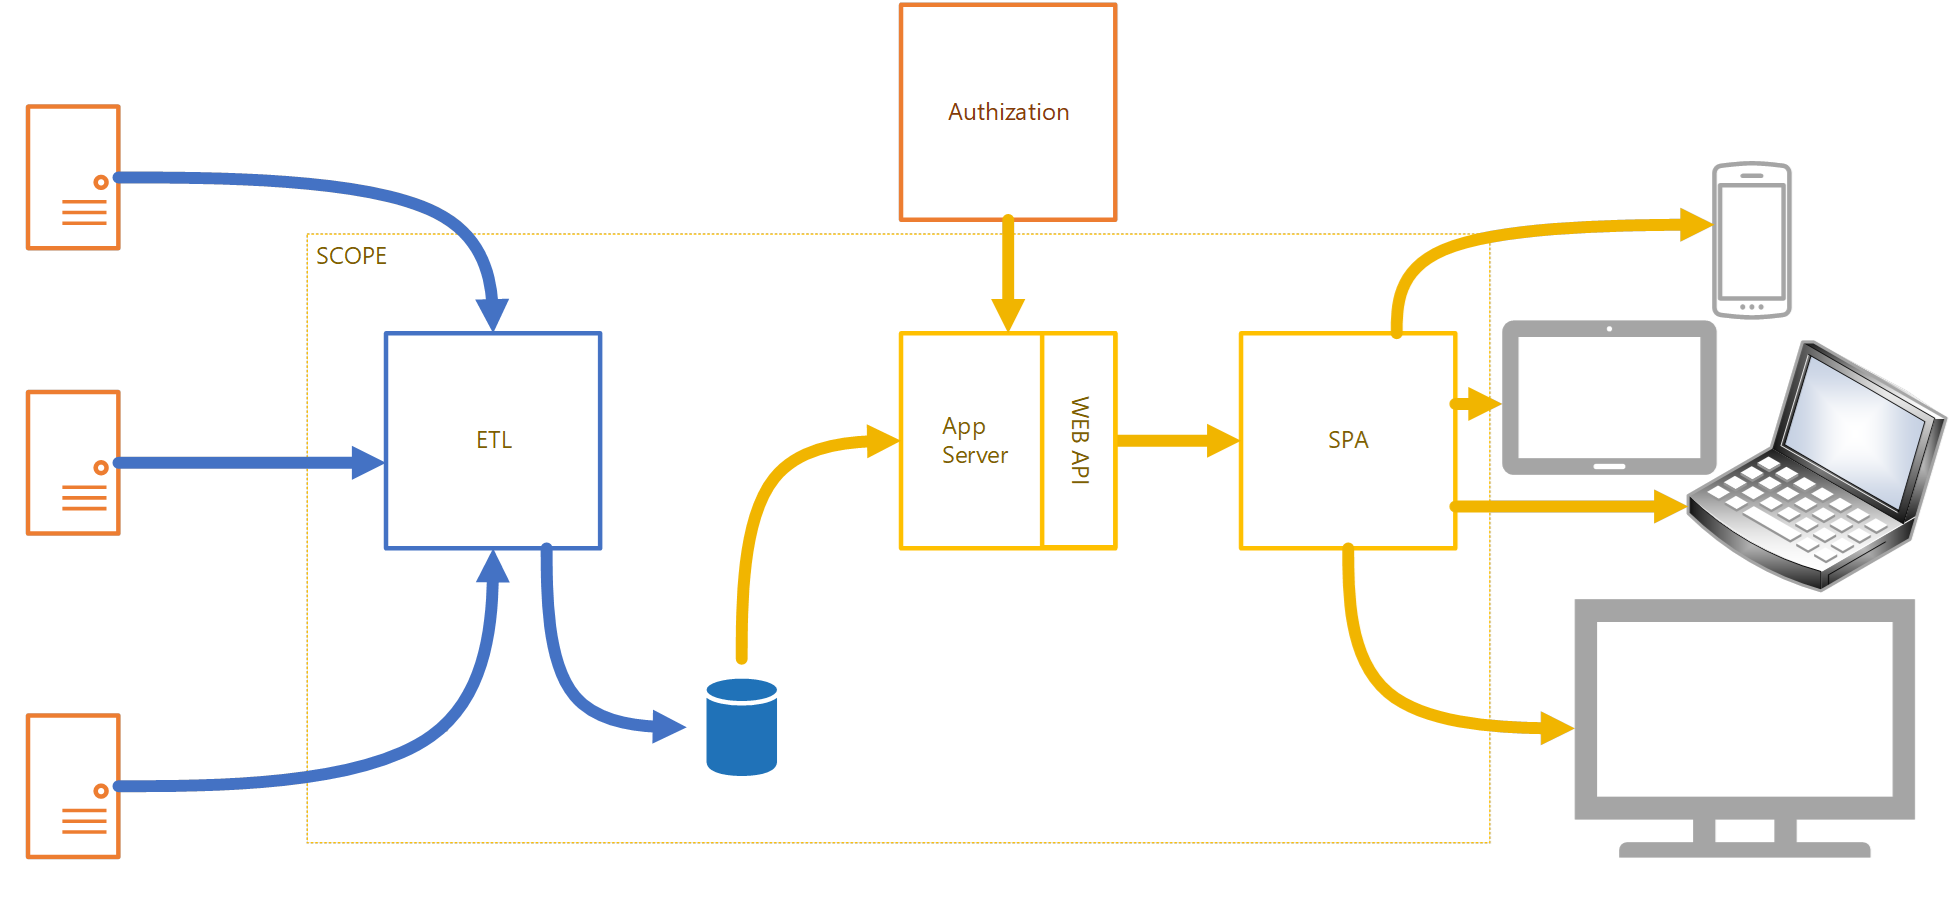
\includegraphics[width=\textwidth]{lean-dashboard-software-architecture.png}
  \caption{Lean Dashboard's Software Architecture and component interactions}
\end{figure}
In Figure 3.1 it is depicted the various components of our application interacting with each other.

The rightmost part represents the information sources. These sources provide its users with an Application Programming Interface (API), this API will be used by the ETL to obtain solely the needed information.

This information can take different forms. The data objects received from the APIs will differ in terms of structure and information, for example, a project is different from an issue. This means it is crucial to implement an optimized Extract module within the ETL component of our application.

After extracting this information, the ETL will send it towards its respective Transformation module, where it will be treated and converted into a new data object with the necessary fields to represent it visually later.

The Load module of the ETL will grab this newly created Widget object and load it on a database.

The ETL procedure is constantly running and updating the existing widgets on the database, according to the widget's time settings that will be presented in this document.

In the middle of the scheme is the core of the application, the Web Server, and its API.

The Web Server is responsible for processing the requests that are sent by the Single Page Application (SPA), as well as managing the NoSQL database running on ElasticSearch\cite{ES}.
It interacts with an authorization and authentication module, the Authization module, to manage the users and their roles within the application.

The API supports a varied range of operations that can be called by the user to manipulate the information inside the database. It presents the user with methods to obtain, create, update, and delete the information in the database.
The API's endpoints can be found with more depth within Appendix A present in this document.

Lastly on the rightmost side of the diagram, there is the SPA, the component that will be accessed by the application user on their preferred device. To provide the user with the best experience, this SPA was developed as a mobile-first, responsive web application capable of supporting different types of display screens, starting from the smartphone up to the bigger ones like a regular desktop computer or a TV screen.

\chapter{Server Implementation}
\section{Scheme of the back-end and Extract, Transform and Load}
\begin{figure}[h!]
\center
  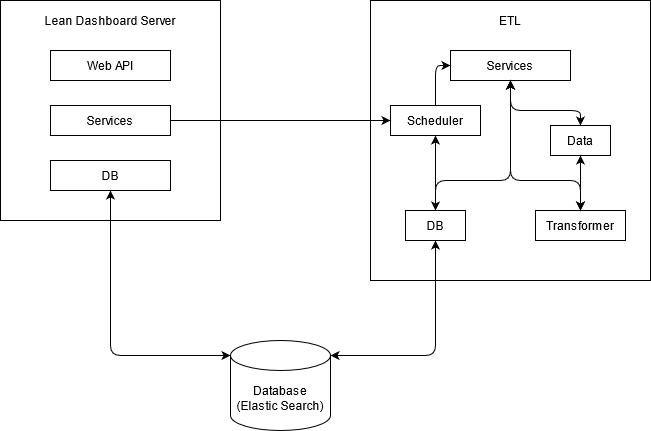
\includegraphics[width=\textwidth]{arquitetura software.png}
  \caption{Back-end structure and modules interactions}
\end{figure}
Figure 3.2 depicts the application's back-end and the information flow between its main components. On the left, we have the Lean Dashboard Server and, on the right, the ETL Procedure, the two key components of the application's back-end.

These two components interact with one another so that the ETL knows what sort of information it should obtain.

The Lean Dashboard Server is composed of 3 Node.JS\cite{NODE} modules:
\begin{itemize}
 \item The Web API module is responsible for catching the requests sent to the API, filtering the parameters and body fields, and sending them to the Services module.
 \item The services module will process every request the Web API receives and forms a function call to the Database(DB) module. If the request consists of modifying or creating a Widget object it will make a call towards the Scheduler module in the ETL.
 \item The DB module is responsible to access and modify the ElasticSearch based database, containing all the necessary functions to create, obtain, delete, and edit the database. It also verifies if the inputted parameters are valid within the context of the application, preventing the existence of duplicates or the association of members to a project who aren't registered in the application, for example.
\end{itemize}
\newpage
The ETL component, as we already mentioned, is responsible for accessing the various data sources and transforming them into a specific widget object.

It contains 5 Node.JS modules in its structure:
\begin{itemize}
 \item The Scheduler module, accessed by the lean-Services module, is responsible for scheduling the automatic ETL process that will update the created widgets according to the time settings a user provides. It accesses the DB module to retrieve the necessary information to execute the correct Services function.

The module is implemented using the node-cron\cite{NODECRON} module so that we can easily create and configure jobs to execute at a set time.
It contains 2 Map objects with distinct functionalities, the widgetMap is responsible for providing the scheduler with the necessary ETL-Services function to execute for the various widgets according to the function parameter contained within the widget's structure, and the widgetJobs associates a widgetId to its currently running job so that we can reconfigure them later.
 \item The ETL-Services module acts as a coordinator for the ETL procedure, it obtains the necessary filtered data from the Data module and then gets the transformed information from the Transformer module.

After the process of obtaining information is complete it calls the DB module so that this information can be stored.
 \item The Data module's task is accessing the selected information sources, currently Azure, Jira, and Squash, and sending them to the Transformer module for some light filtering, returning the retrieved object with only the necessary information for its transformation.
 \item The Transformer module's job is to transform the data into the required information for the widget to be displayed. It transforms the data into widgets such as a Pie Chart, a Data Table, or a Gauge Chart.
 \item Finally, the DB module is responsible for updating the widget's information with the updated data obtained from the ETL procedure.
\end{itemize}

\newpage
\section{Data Model}
For the Data model and the storage of the information, we chose the No-SQL database Elastic Search.
 
To better facilitate the getting and storage of information, we divided each object into its own index, as displayed in the following scheme:

\begin{figure}[h!]
  \center
  \resizebox{120mm}{!}{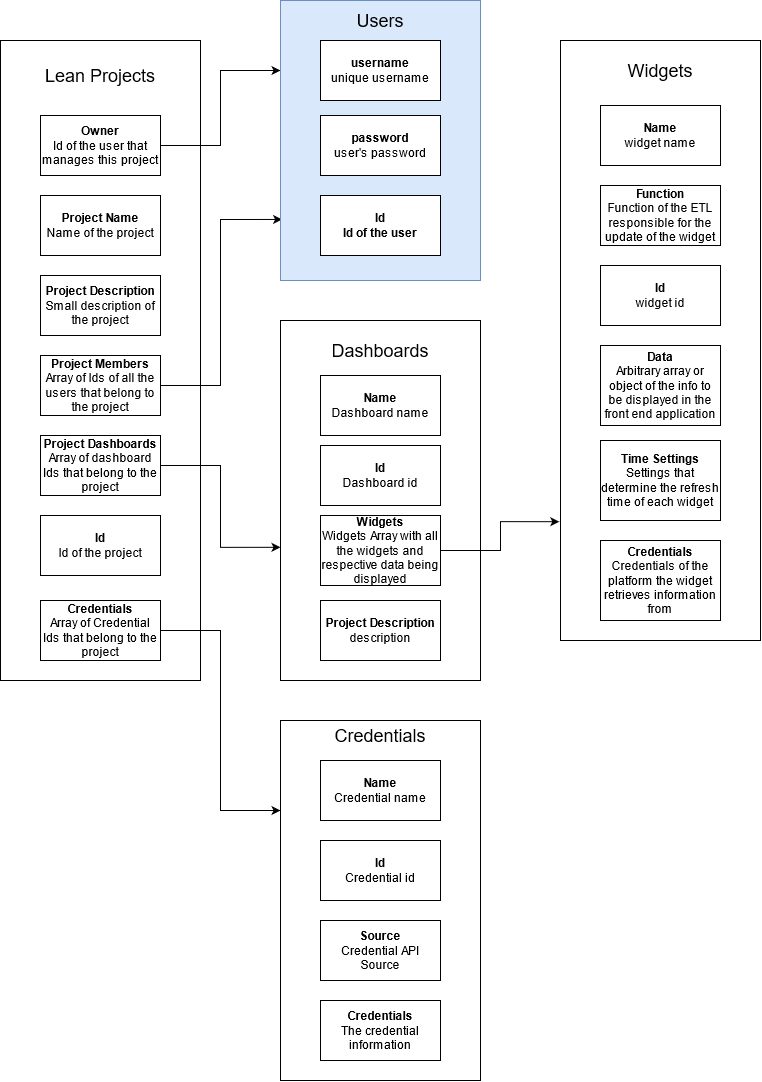
\includegraphics[width=\textwidth]{modelo de dados.png}}
  \caption{Database Data Model}
\end{figure}

Figure 3.3 depicts the application's data model and the object's structures. Each of these objects contains the necessary fields to store the needed information for the application. 
\newpage
Each object is detailed as the following:
\newline

\textbf{Lean Projects}

This is the index where all the Projects created with our application are stored, acting as the main gatherer of information.

It has information over who created it (Owner), the Project's name, its description, and a unique identifier.

Each project can contain a varied number of members, dashboards, and credentials. 

This information is stored inside an Array of identifiers, these being Project Members for the members that are currently associated with the project, Project Dashboards for the dashboards, and Credentials for the credentials.

The members simply act as viewers of the information within the project, they can only access dashboards and view the information on the widgets.


\textbf{Users}

The users are highlighted in a different colour on the scheme to better differentiate them from the data model since they aren't being stored in the database our application manages and are being stored in the Authization module's database.

Each user will have a username and a password so they can log in to our application, as well as a unique identifier within the database to be used by the array of members within the Lean Projects Objects.


\textbf{Dashboards}

The dashboards are where the widgets will be stored. They don't exist if there isn't at least an already existing Lean Project and will be presented as a web page with all the widgets within the dashboard being displayed.

The dashboard objects contain a name, an Array of Widget identifiers that are associated with the dashboard, a description, and a unique identifier within the database.


\textbf{Credentials}

The credentials consist of a specific object containing a name, a source (Azure, Jira, or Squash), and a credential object containing all the credentials themselves.

This credential object is structured as such for each of the information sources:

\begin{figure}[h!]
\center
  \resizebox{120mm}{!}{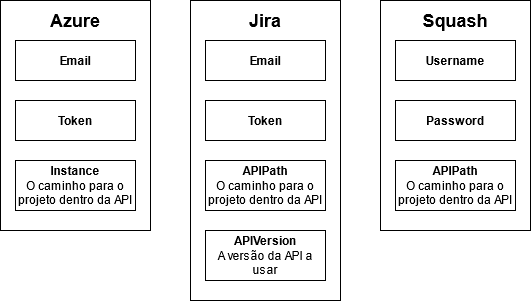
\includegraphics[width=\textwidth]{formato das credentials.png}}
\caption{Credentials and their structure for each data source}
\end{figure}

Each source requires a different form of credential so that the authentication on their web API is successful. These credentials are mandatory as the ETL procedure cannot access the specified information source's API without them.
\newline
According to figure 3.4:
\newline

Azure requires an email, a token, and an Instance field related to the project within the API.

Jira requires an email, a token, an APIPath for the project within the API, and an APIVersion that refers to the API version to be used.

Squash only requires a username, a password, and the APIPath.

\newpage

\textbf{Widgets}

The widgets are the result of the ETL procedure.

They are created by the user through the selection of a widget template that will serve as a widget with temporary data to be displayed.

Widgets consist of several fields like a name, a function, a data object, the time settings for the ETL schedule, the required credentials, and a unique identifier.

The function field refers to which ETL function the scheduler needs to call to start the node job.

The time settings are an object that contains information related to the interval at which the ETL procedure is executed to update the widget. 

Each field of this object is structured in CronTab format and consists of:
\begin{itemize}
 \item seconds;
 \item minutes;
 \item hours;
 \item day of the month;
 \item month;
 \item day of the week;
\end{itemize}
The credentials are the credential object associated with the project.

Without them obtaining information is impossible, making it a required field when creating the widget.

The data object is where all the transformed ETL information will be stored. It is the main reason the application utilizes an ElasticSearch database, as the information contained within this object will vary from widget to widget, making it a hard task to store consistently within a relational database like PostgreSQL.


\newpage
\section{Authization module, Backoffice and Access control}
 To give our users authorization and authentication features we had to think of a way of letting users create accounts, have users with different roles inside the application, and have different roles have their privileges. To give users that set of features, and as a request of Inetum, we utilized a Node module called Authization\cite{AUTHIZATION}. 

As a reference point, this module was a project developed last year by the ISEL students Tiago Matias, Diogo Leandro, and João Barata of the LEIC programme as a final project of the Project and Seminar course, and was also developed in partnership with Inetum, and serves as a module that allows to set up an RBAC model with various roles, permissions and decide which roles should have access to what permissions. The module will also take care of aspects such as login, logout, and the creation of users. Since the module requires a SQL Database for the storage of users, we had to use PostgreSQL\cite{POSTGRESQL} to handle the storage of users, the created roles, and permissions.

As for the RBAC model, it was requested that there were three types of users: a master user, with every kind of access and ultimate control (that includes access to every existing project, both seeing and editing them), a user that would be able to manage certain projects and create new ones and finally a user with only permission to see projects he is a part of.
With that said, we came up with an RBAC model with the roles Superuser, Manager, and Collaborator, with the following accesses:
 

\begin{figure}[h!]
\center
  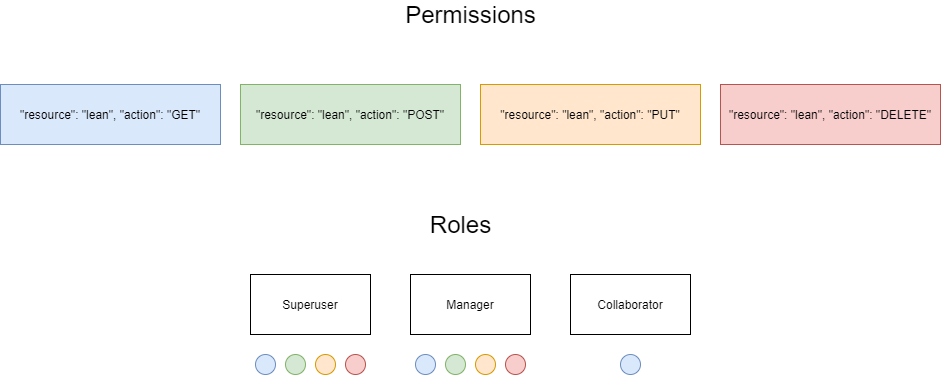
\includegraphics[width=\textwidth]{lean-rbac-model.png}
\caption{Application User Roles and their respective permissions}
\end{figure}
As said before, we defined three roles. The Superuser will have access to all the defined permissions, being able to access and modify all projects, without having to be a part of them. 
Below the Superuser, the Manager role will act in a similar way to the Superuser but will only be able to modify projects that we're created by himself. Additionally, he will only be able to visualize projects (and the dashboards and widgets associated with the said project) if he is a member or instead, the creator of that project. A manager will be able to manage aspects of a project such as its name, description, containing dashboards and widgets, as well as all the members in it.
Finally, the role of Collaborator. Being the role with fewer permissions, users with this role will only be able to access projects they are members of.

\chapter{User Experience Research}
This section covers our User Experience research and studies on how our application should be controlled.

Our research on every necessary item to develop an application that is easy and intuitive to use will be presented here.

User Experience, commonly called UX, is the term used when referring to how users interact with a certain product. If we use an analogy, if we were to open a door, it is more about how the door handle is used than what shape or colour it has, or what material it is made from. 

UX is also greatly impacted by the context a product is being used and the type of users using said product. Inetum conducted UX research using contextual interviews with potential users of Lean Dashboard to understand their real needs. After studying the observations, 2 Personas were created that focus on the needs of the real target. That list of personas would help us take into consideration how we would address the UX design of our early digital prototypes (which later reflect on the client application), by having various types of users with specific personalities, most wanted features, and specific positions inside a company. 

Following that, we developed a digital prototype that would allow us to make a series of usability tests with real users. Those tests would allow us to better determine what needed to be addressed in our digital prototype and solve issues before any implementation was being done.

With that said, we believe the User Experience research done by the group is something that can greatly improve the result of the client application, whilst saving implementation time by allowing us to make some decisions beforehand. Usually, problems are easier to solve in a digital prototype than they are in code.

\section{Red routes diagram}
A Red Routes matrix is developed to aid a designer to identify the crucial and frequent tasks which users perform with our product. It consists of a matrix that delivers the frequency of performing, as well as the number of users who perform a specific task.
 
In the process of identifying Red Routes, there are some factors to be considered:
\begin{itemize}
	\item Critical: Tasks that deliver relevant value to users.
 	\item Frequency: Tasks that are performed at high frequency, usually represent the use cases of over 90\% of users.
 	\item Key-value drivers: Red Routes drive the key business metrics.
 	\item Impact: Red Routes significantly affects the overall user experience.
\end{itemize}
Through identification of our users' top tasks, we can:
\begin{itemize}
	\item Foresee users' needs.
	\item Develop a website utilizing users' needs.
	\item Target fundamental website pages.
	\item Conduct usability tests.
\end{itemize}	
Regarding the identification of Red Routes' major advantage, it aids the team to identify the most important content and functionality rooted in usefulness to most users. Further, it supports a team in the selection of the minimum viable product (MVP), which leads to a more significant product roadmap design with the purpose of continuous iteration and overcome potential usability barriers on relevant user journeys. 
\begin{figure}[h!]
\center
  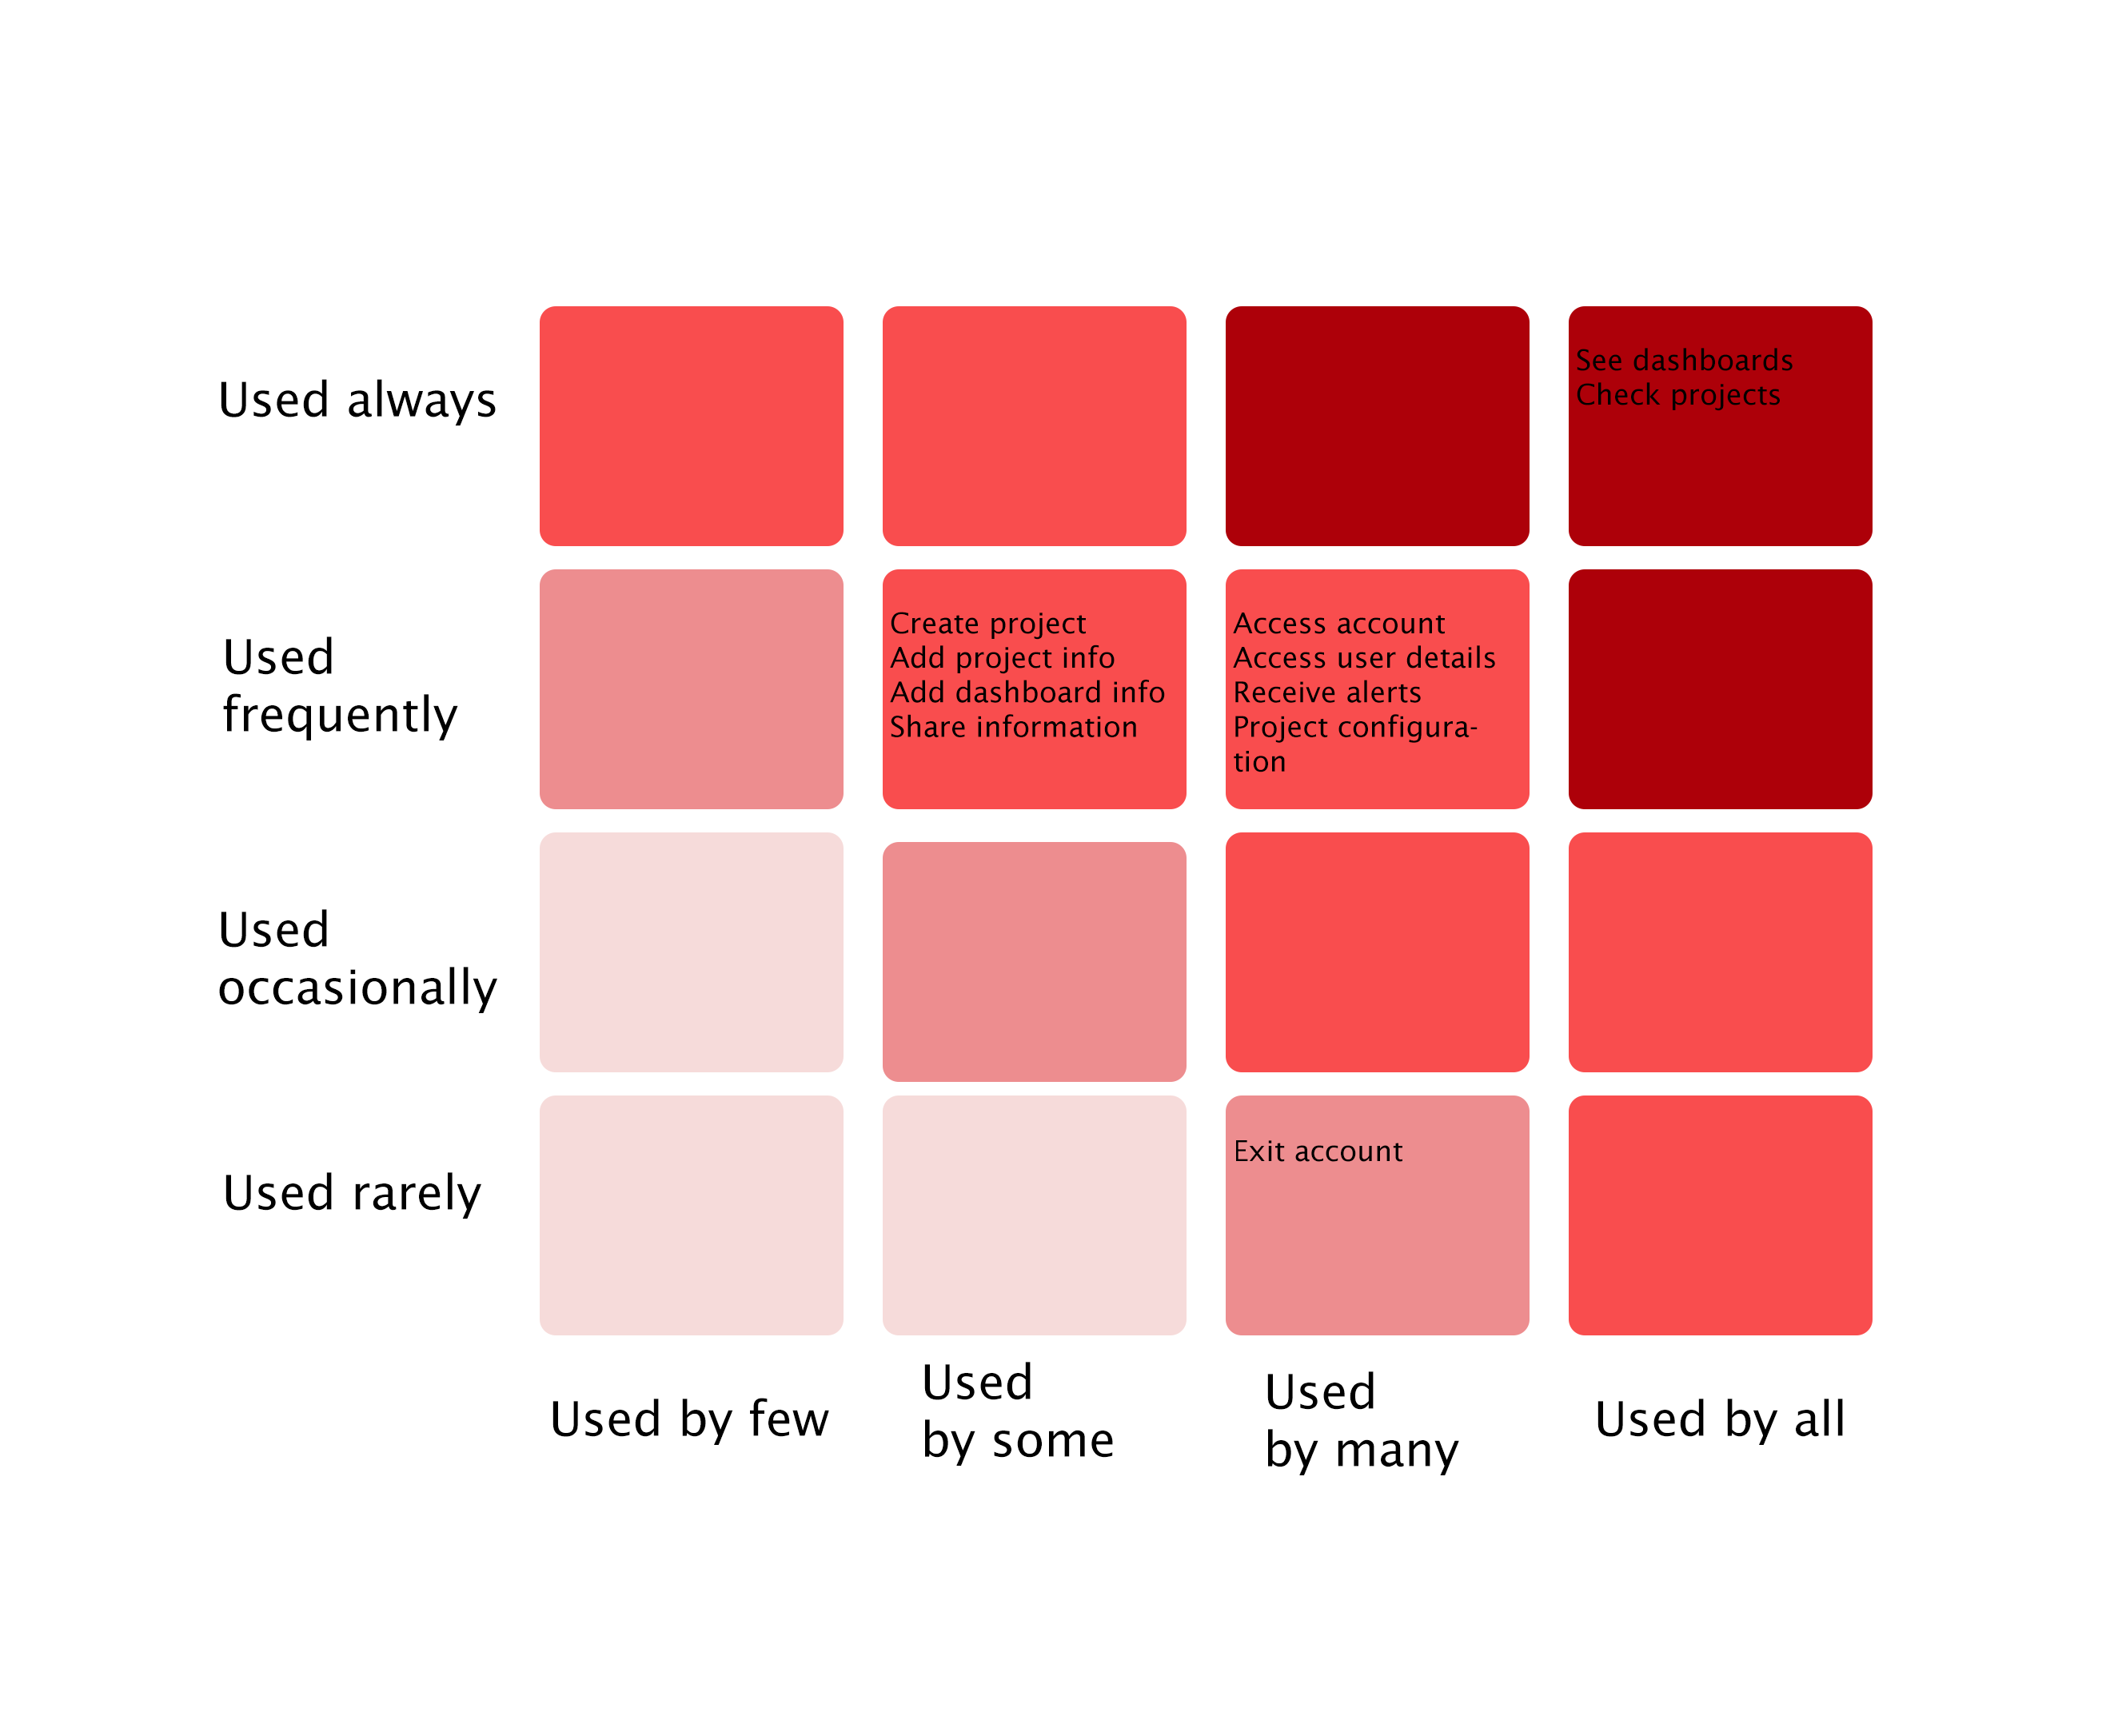
\includegraphics[width=\textwidth]{red-routes.png}
\caption{Red Routes Diagram}
\end{figure}

The team designed the Red Routes for the Lean Dashboard application, as we can see in figure 4.1, based on the list of Personas that Inetum provided. We considered the above factors to create the Red Routes in the best way possible.
\newpage

\section{Information Architecture}
Information architecture (IA) consists of the capability of sorting and designing the content of not only the web but also websites and mobile applications. 
The main purpose of information architecture is to organize content to facilitate the users' process of tuning to the product's functionality and thus, finding anything they might want easily.
There are several elements that can affect the content structure, among which, IA experts tend to regard the specifics of the target audience's needs. This can be justified by the fact that the IA prioritizes user satisfaction.
The main factor that leads people to visit different websites is content. It is commonly shared that producing valuable content for users is crucial, but so is ensuring that the content is easily found. We use Personas that Inetum provided as a tool to find the most adequate IA and run usability tests.
 
\begin{figure}[h!]
\center
  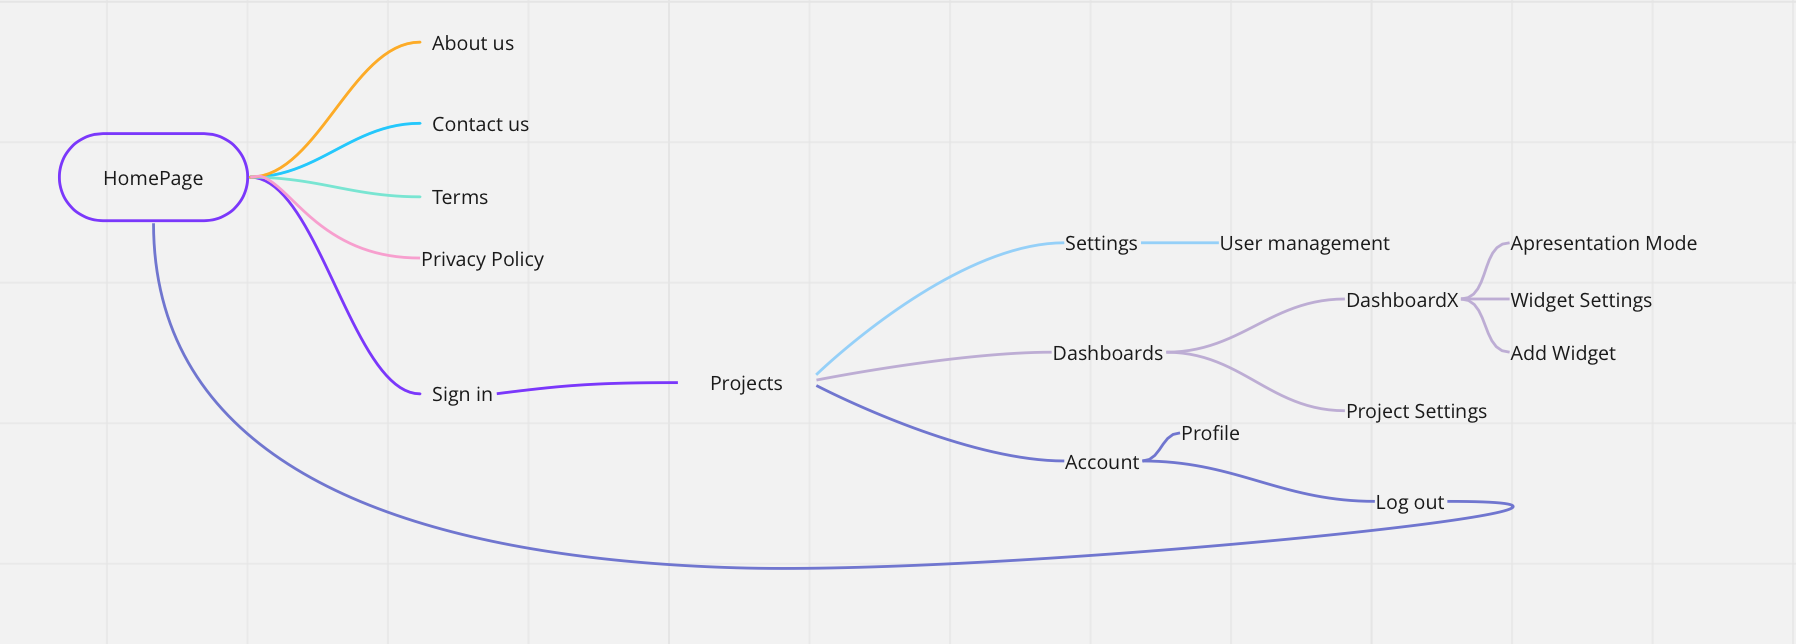
\includegraphics[width=\textwidth]{information-architecture.png}
\caption{Information Architecture Diagram}
\end{figure}

With this diagram, we can better plan the making to the various resources by achieving a flowchart that dictates if the various flowchart accesses make sense (and easily correct them if they don't).

\newpage
\section{Digital Prototype and Usability Tests}
A Digital Prototype is a tool used in UX research to develop a mock user interface that can be utilized in use-case tests. These tests gather a small group of people and establish a task that all users need to complete. 
 
A Digital Prototype is how we validate our basic idea and the premises underpinning it by collecting user feedback.
With the obtained results, we can then determine what aspects need to be addressed in the Digital Prototype by us developed.

The usability tests were performed by five Inetum employees, the team used five simple use-cases to test the digital prototype. The use-cases that were used: 
 \begin{itemize}
	\item USE CASE 1: A user creates a Lean Dashboard account and creates a project. Then log out of your account.
	\item USE CASE 2: A user already with an account created, creates a dashboard in an existing project.
	\item USE CASE 3: A user with an account created creates a widget in an existing project and dashboard.
	\item USE CASE 4: A user already with an account created, adds a member to his existing project.
	\item USE CASE 5: A user already with an account created, changes the project name.
\end{itemize}	

After performing all tests, the team changed some web flows, buttons and created new pages based on the interviewee's feedback. 

This research and planning done beforehand (before the full implementation of the client application) can greatly decrease implementation costs since it is much easier to make modifications to this mocked user interface than it is to make some of the same changes on the client application code.
We utilized the platform Figma\cite{FIGMA} to develop our Digital Prototype on figure 4.3:
 
\begin{figure}[h!]
\center
  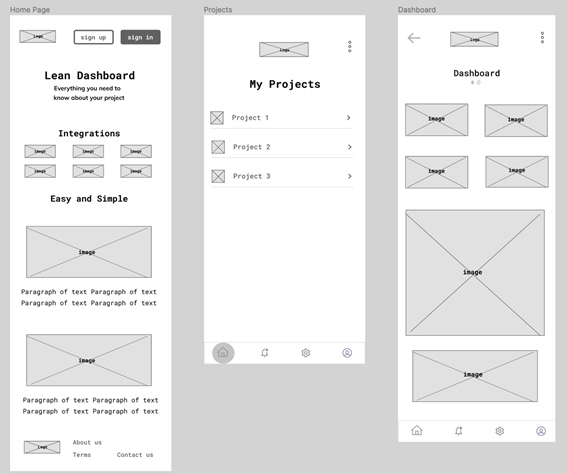
\includegraphics[width=\textwidth]{digital-prototype.png}
\caption{Application Digital Prototype}
\end{figure}

\chapter{Client Implementation}
The following chapter explains the implementation for the client’s side of the application. 

This section, it is mostly explained the decisions made when implementing the client application, as well as what each page of the application is used for and how they function.
 
\section{React vs Angular}
React was our choice over Angular. The reason behind such a decision was that Angular has a lot of concepts and syntax to learn, as well as the fact that Angular's documentation is much longer, and we believe it might take some time to learn a new language given that the time frame is relatively short. React is easier to learn in the short term than Angular and the group that developed this project would attend a course to learn react, which would be an asset.

React is an open-source JavaScript library focused on the development of user interfaces. With this library developing web applications, SPA (Single Page Application), or mobile applications turns into a very easy task since it offers great benefits in modularity and promotes a very clear flow of data and events. This greatly facilitates the development and planning of complex apps.
We make use of the React Router library for the routing of the application. It enables the navigation among views of various components in a React Application and keeps the user interface in sync with the URL. It greatly helps with developing the application's navigation and how each page should look like.

\section{React Hooks}
React has very powerful tools to use when writing code for an application. These tools are known as "Hooks".

Hooks are functions that allow us to “hook into” React state and lifecycle features from function components. Most of the hooks are built-in with the React library. By using these Hooks, we can use state and other React features without writing a class.

Since we ended up using the React technology for the development of the application front end, it is essential to give shed some details about the most important Hooks we used.
\newline
On our client application we use 4 main hooks, these being:
\newpage
 \begin{itemize}
	\item useState\cite{USESTATE}:

This hook is used to store the state within our components. Throughout the application, we mostly used it to save the data we fetch from our API and the input for the application, but also to save information regarding the user rules (for example, if the user logged in as a manager, that information will be saved in state variable when the user is checking it profiles).
	\item useEffect\cite{USEEFFECT}:

useEffect is a hook that allows us to run and control certain effects on our components. The effect is run whenever a component is loaded or when the data in one of the dependencies is changed. In the context of our application, we use this hook to run the necessary functions to obtain data from the API and store it in the state.
	\item useContext\cite{USECONTEXT}:

This hook is used to store the context within our application. Within our application, we use it to save the session context of the application. Whenever a user logs on to the application, their credentials are stored as context, and it is used to ensure the user is still logged onto the application.
	\item useFetch\cite{USEFETCH}: useFetch is a custom hook that allows us to make fetch requests to our API.
\end{itemize}

\section{Client Architecture}
\begin{figure}[h!]
\center
  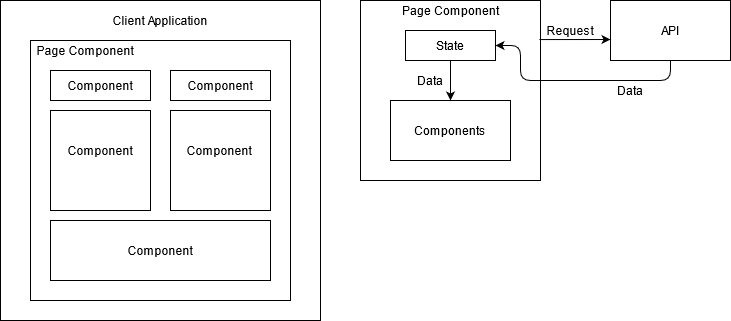
\includegraphics[width=\textwidth]{client app architecture.png}
\caption{Application Components and Data Fetch}
\end{figure}
On Figure 5.1 is our client's structure. 

On the leftmost part of the diagram, we have the component organization, these can be distinguished by page components and regular components.
The page component is where all the smaller components are organized. 
\newline
The page component is also the one responsible for making the requests to the API and save the data on the state, as shown on the rightmost part of the diagram.
\newline
The state is then passed down to the regular components so they can display the necessary data to the user.
The regular components can be reused on various page components.

\newpage
\begin{figure}[h!]
\center
  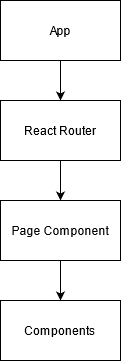
\includegraphics{client app interations.png}
\caption{Application Data Flow}
\end{figure}
Figure 5.2 is the data flow of our application.
The App is the main entrance to our application, this is where the routing and session context verification is done.
The app accesses the React Router to define the necessary URL for the application, depending on the URL the Router provides the user with the specific page component if the user stored context with useContext has valid credentials.

\section{Pages and Components}
Components are the building blocks of the React app. The components is a JavaScript function that optionally accepts properties and returns a React element that describes how a section of the User Interface should appear on the user screen. 

Inside the Pages directory, we have the web pages where interact with the server and provide data for the components. This package contains the views of the general pages and uses the components to create these pages. 
\newpage

\section{Client Side Widgets}

Widgets are among the most important parts of our application. They are how the information obtained from the various APIs will be displayed.
\newline
As such each type of widget we support is its separate component. 
\newline
We provide 4 types of different widgets:
 \begin{itemize}
	\item Bar Chart
	\item Data Table
	\item Gauge Chart
	\item Pie Chart
\end{itemize}
These widgets were developed in such a way that can adapt to any form of data that is sent to them, for example, the Data Table will have the necessary columns to display the data and the Pie Chart will have as many divisions as required. To help the creation of the charts we use packages like react-chartjs-2 and react-gauge-chart. 

\section{Client Side Access Control}
To keep in line with the rules of access to each project and its dashboards, in each project and dashboard a given user tries to access, a set of verifications are put inset.

Usually, a list of the user's projects is shown right after the login, and the user chooses which project it wants to interact with and see all its dashboards by clicking on it:
\begin{figure}[h!]
\center
  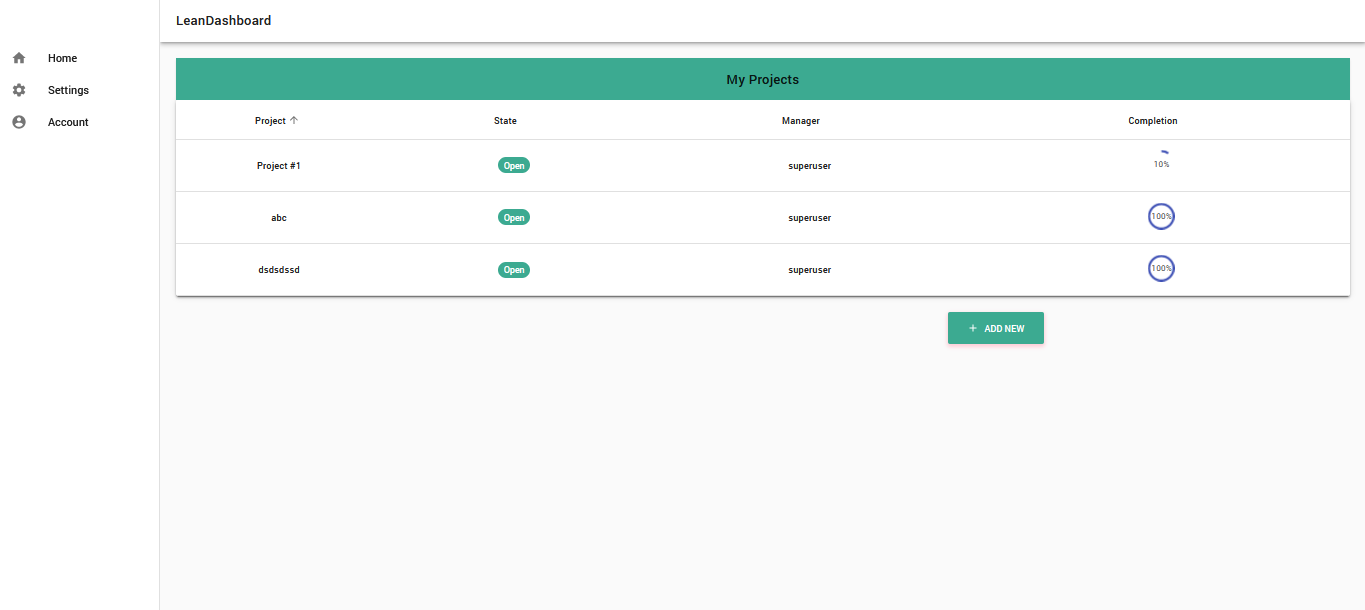
\includegraphics[width=\textwidth]{projectsPage.png}
\caption{Projects page presented to every user after logging in}
\end{figure}

The projects presented in that list only include the projects the user is allowed to see, and thus no further verification is necessary.
However, a user can try and access a specific project’s dashboards by typing the entire URL. To control possible illegal accesses, we must verify the result of each request made:
\begin{figure}[h!]
\center
  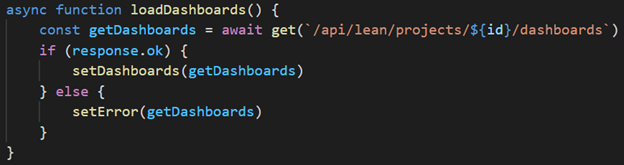
\includegraphics[width=\textwidth]{load-projects.png}
\caption{Function responsible for fetching all the projects}
\end{figure}

Using the react hook use-http (the hook used for all the requests to the server) we fetch all the project’s dashboards.
Depending on the result, the page shown to the user can be the project’s corresponding dashboards, in case of a successful request:
\begin{figure}[h!]
\center
  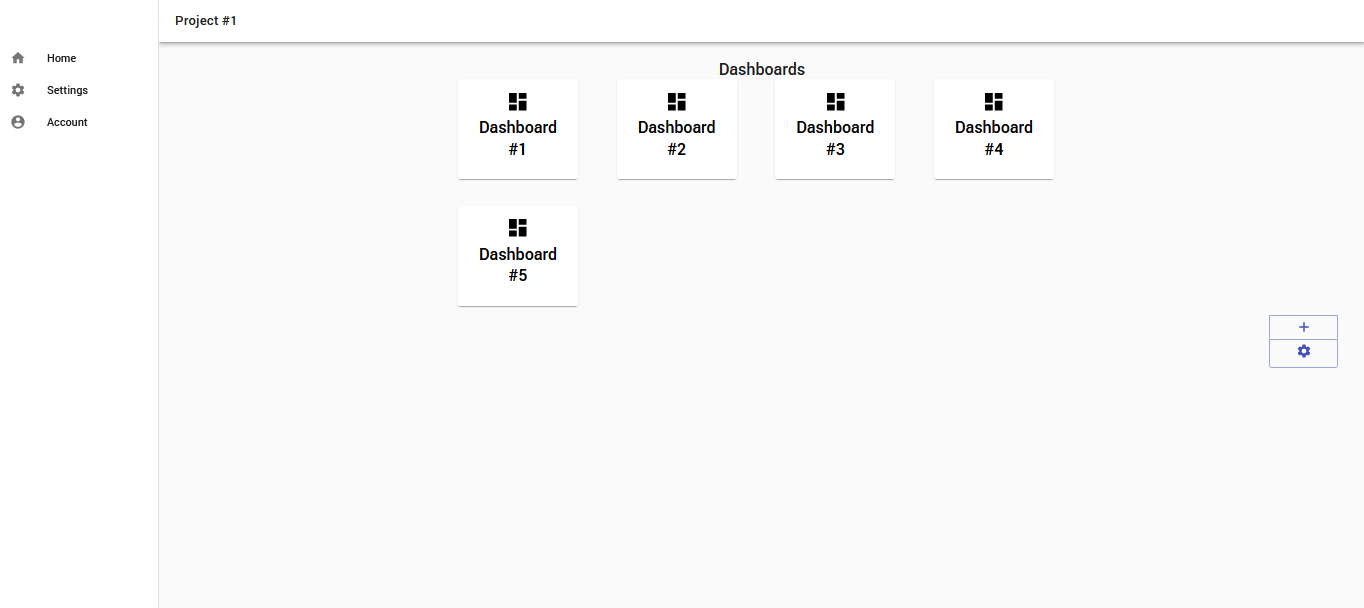
\includegraphics[width=\textwidth]{dashboardsPage.png}
\caption{The dashboards page shown to a user, after selecting a specific project}
\end{figure}

\newpage
Otherwise, the user will be greeted with an error page, in case it tries to see the dashboards of a project it doesn't have access to:

\begin{figure}[h!]
\center
  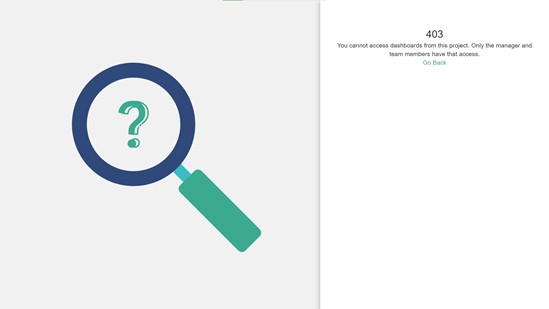
\includegraphics[width=\textwidth]{error-403.png}
\caption{Error page shown to a user when trying to access a project it doesn't have access to}
\end{figure}

Additionally, if a user tries to access a specific dashboard’s widgets by manually entering the URL, the application will have the same behavior and display an error page.

Since there are different roles in this application (collaborators, managers, and one superuser) it is necessary to impose a set of restrictions when it comes to the various permissions (such as create and delete projects and dashboards, manage users, editing widgets...).

For example, the projects page will vary whether the user logged in is or not a manager. A regular user will not have an Add Button, since it does not have that permission, only managers and the superuser do:
\begin{figure}[h!]
\center
  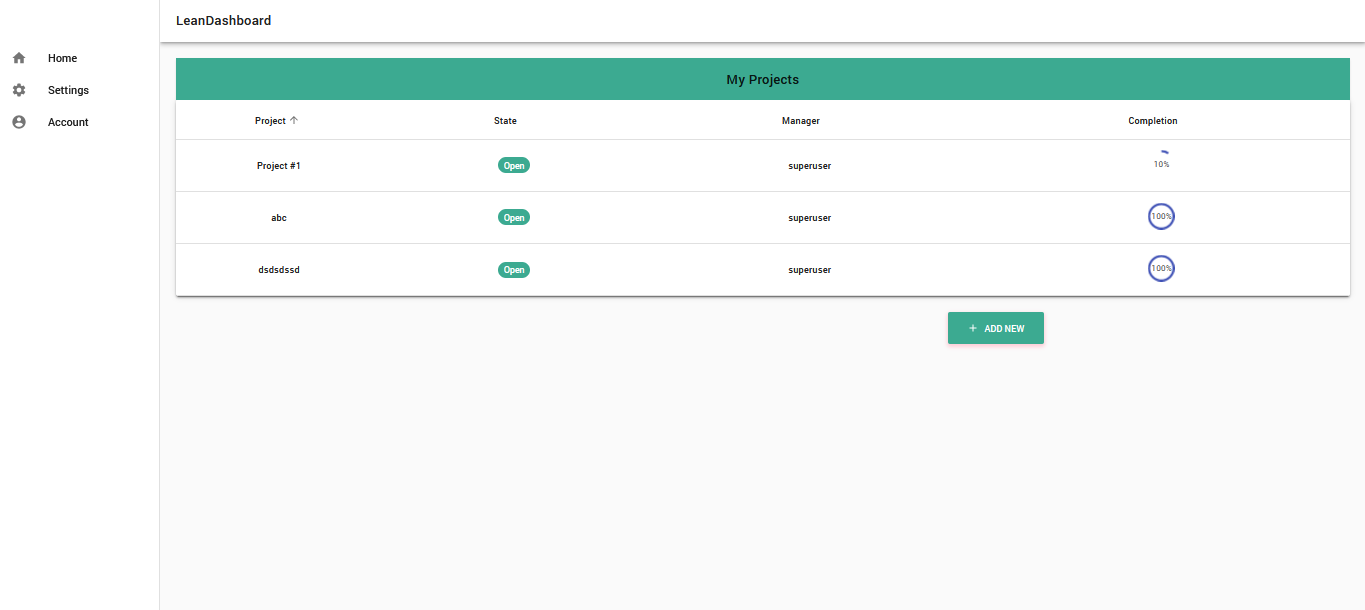
\includegraphics[width=\textwidth]{projectsPage.png}
\caption{Projects page with the "Add Button", presented to managers and the superuser }
\end{figure}

\begin{figure}[h!]
\center
  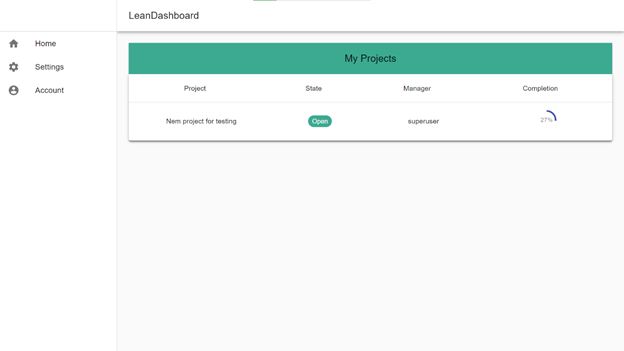
\includegraphics[width=\textwidth]{projectsPageNoAddButton.png}
\caption{Projects page without the "Add Button", presented to all collaborators}
\end{figure}

\pagebreak
This verification however requires an extra request from the API: 
\begin{figure}[h!]
\center
  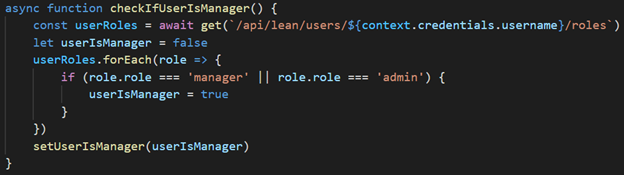
\includegraphics[width=\textwidth]{checkIfUserIsManager.png}
\caption{Function responsible for fetching all the user's roles and check if the user is or not a manager or the superuser}
\end{figure}

\newpage
Here, we use the context (in this case, the context is the React hook useContext) which stores the current user logged in and once we have its username, we make a get request for the user's roles. 
If the current user happens to be a manager or a superuser, we use the react hook useState to set the Boolean state variable userIsManager variable with true. The button will then be available for the addition of new projects.
The same method is used to verify if a user can access the back-office page. Whenever a user accesses the settings page, the same verification is made and only the superuser and managers will see the button to access the back-office page:

\begin{figure}[h!]
\center
  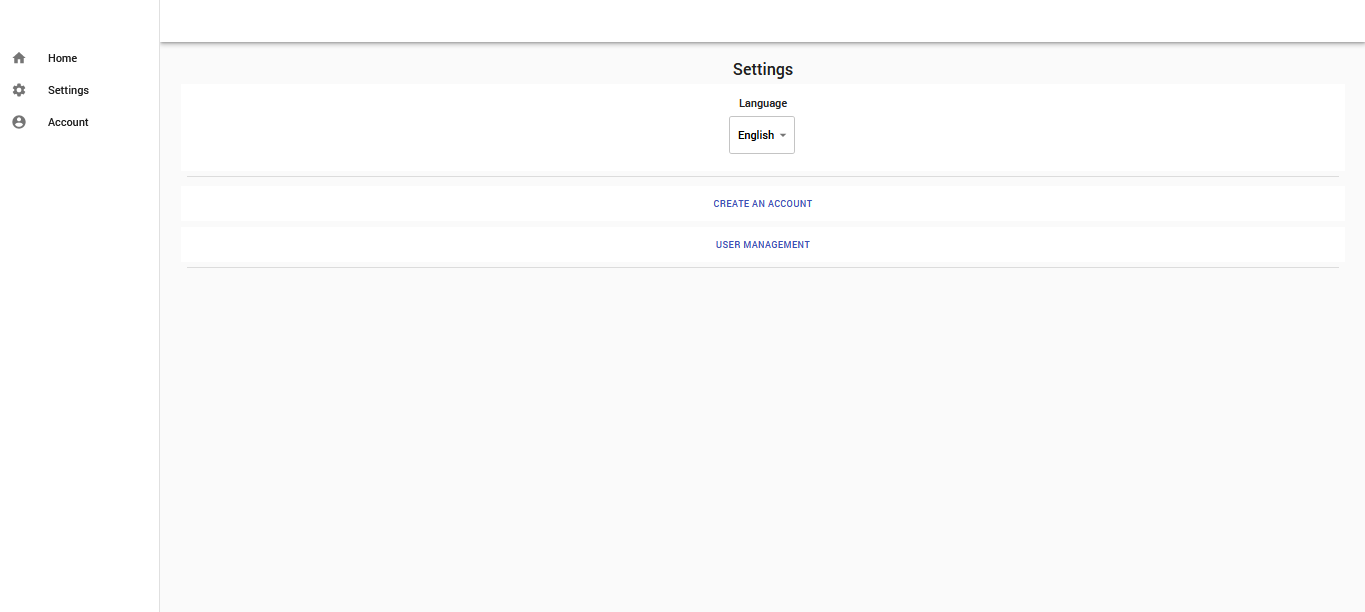
\includegraphics[width=\textwidth]{settingsPage.png}
\caption{Settings page presented to managers and the superuser}
\end{figure}

\begin{figure}[h!]
\center
  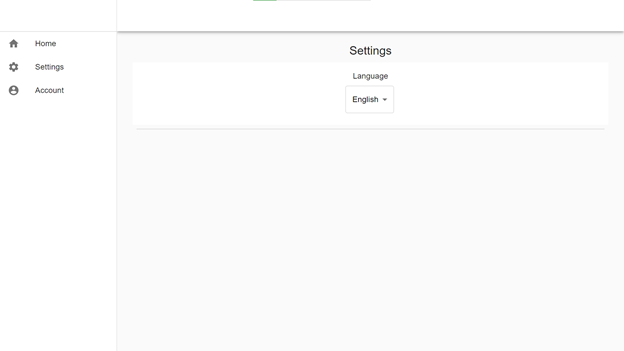
\includegraphics[width=\textwidth]{settingsPageForCollaborators.png}
\caption{Settings page for all collaborators}
\end{figure}



\chapter{User Interface}
The following section presents the graphical user interface (UI) of the application.
\section{User Interface}
With help from the information gathered from the user experience tests, the front-end application started development using React.
\newline
Based on the low fidelity prototype designed to conduct the tests, we implemented the necessary pages and components for the application.
\newline
Each component is designed in a way that makes recycling them on other pages easier and each page was easily and quickly implemented by using the Material UI Framework, an easy-to-use tool that provides pre-made components.
Material UI also provides methods and tools to design pages according to the screen size being used to view the client application, making implementing the mobile and desktop pages a much simpler task.
\newline
As of now, the client application has multi-language support for 3 languages: English, Portuguese, and French. It uses i18n to translate.
 
\begin{figure}[h!]
\center
  \includegraphics[width=\textwidth]{HomePage.png}
\caption{Home Page}
\end{figure}

In figure 6.1, we have the Home Page, it is the first page the user sees. Here the user can change the language of the application and may begin his Log In process, by pressing the Sign-in button. Once the button is clicked the user will be redirected to the Sign-in page where he will be inserting his credentials to enter the application.


\section{Sign In Page}
The sign-in page is where the user enters the credentials necessary to sign into our application.
They only must input a valid username and its associated password to enter.
\newline
The page has a checkbox the user can toggle to allow the browser to keep track of the session. 
The user's session information is stored in two different storages.
\newline
The session storage is used when the user does not want the browser to remember them since the information is cleared when they close the tab.
\newline
The local storage is used when the user toggles the "Remember Me" checkbox. This storage will save the session information and won't be cleared until the user logs off.
So that this effect can be verified, the application verifies if the browser has any saved session, if it's not saved the client redirects the user to the login page if the user is trying to access a restricted page.
\newline
The user's username is stored within the application by using the React Hook "UseContext" to later be used for the required API calls.
In case the session information is saved, the client sends a request to the API to authenticate the user within the application.

\begin{figure}[h!]
\center
  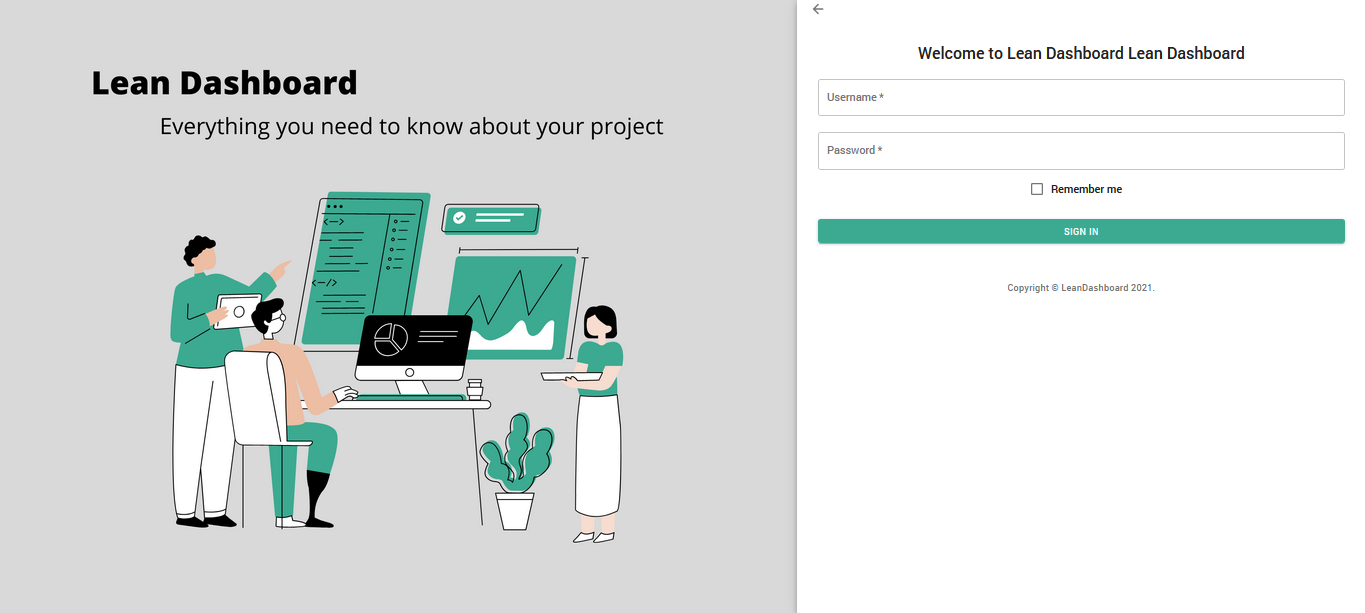
\includegraphics[width=\textwidth]{SignIn.png}
\caption{Sign In}
\end{figure}

\newpage 

In figure 6.2, is the view that represents the entrance to the user account. It is composed by a form of two text input boxes that receive the username and the password.

\section{Projects Page}
This view presents to the user the projects that he is on. The page displays in form of a table or list of the projects composed by name, state, manager, and completion, which is the percentage of completion of the projects. The manager or superuser role can add a project by pressing the button. Once clicked will show up a pop-up to fill with name, description, and end date.

\begin{figure}[h!]
\center
  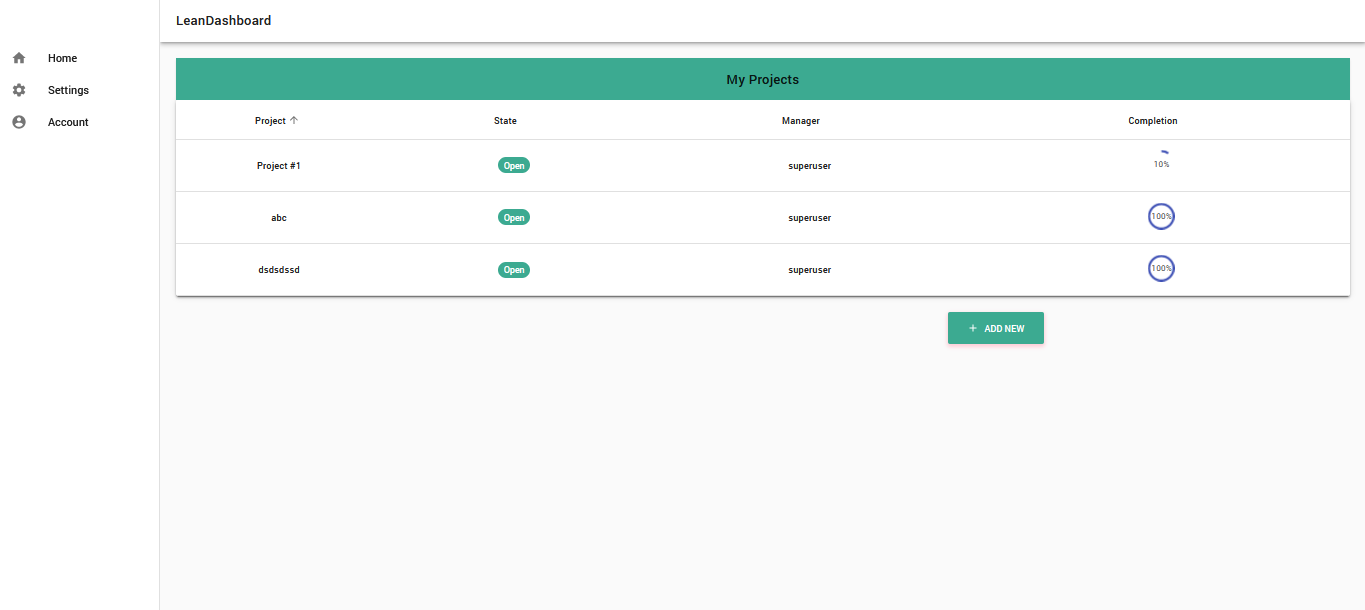
\includegraphics[width=\textwidth]{projectsPage.png}
\caption{Projects Page}
\end{figure}

\section{Dashboards Page}
This page gives the user a view of the dashboards inside of a project. It can be displayed in form of a list or a group of cards. On this page, we can add a dashboard and be redirected to the project's settings page. On mobile, the way that options appear is with a swipeable drawer and for other screens with a group of buttons displayed on the left side of the screen.

\begin{figure}[h!]
\center
  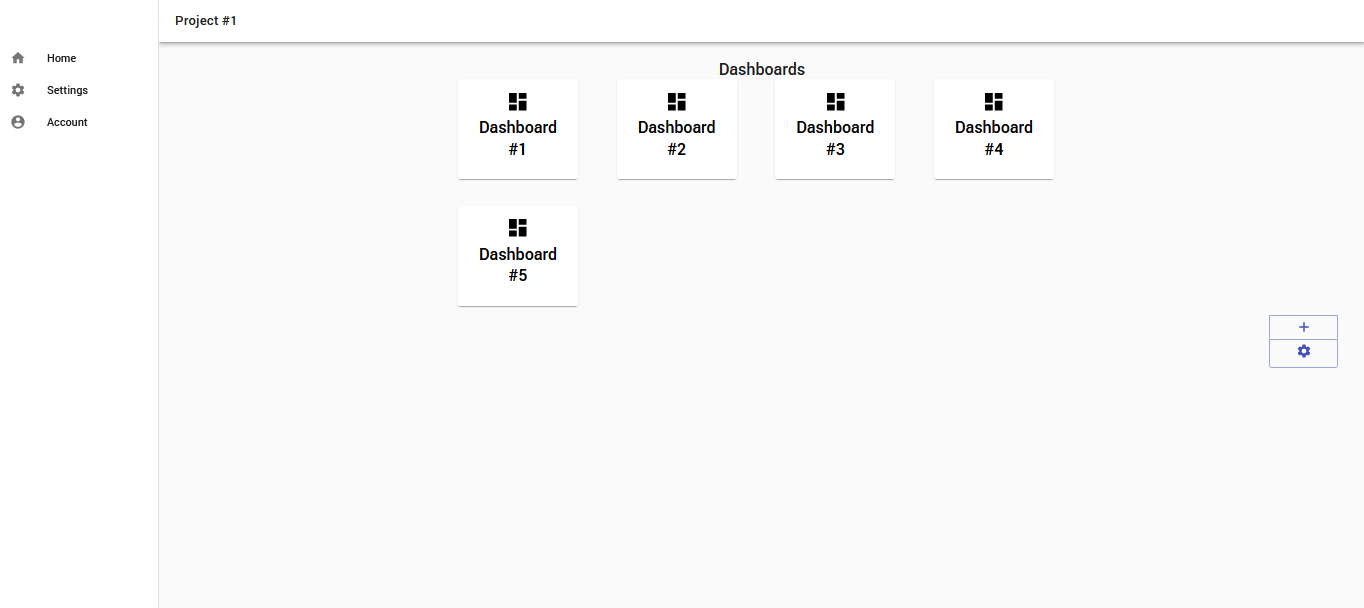
\includegraphics[width=\textwidth]{dashboardsPage.png}
\caption{Dashboards Page}
\end{figure}

\newpage
\section{Dashboard Page}
On this page, the user will see the widgets of one dashboard. This page offers four options in the group of buttons or a swipeable drawer, such as add widgets, dashboard settings, delete a dashboard, and edit widgets.
By clicking on the first option, the user will be redirected to a page where all the template widgets that can be added to Lean Dashboard are presented.
The second option is a pop-up to change the name and description of a dashboard.
The third is a pop-up to delete the dashboard and the fourth button will be redirected to a page like the template widgets to edit a specific widget, like deleting it, changing the credentials being used, or the update time.
\newline
Adding a widget to a dashboard requires the user to select a template from the list of supported widgets. After this has been decided, the user is presented with a dialogue with the required widget information. The user must select credentials according to the source of the widget and the update time settings. When the user edits the time settings, they are presented with a clock if it is a time input or a calendar if it is a date input. When the user confirms this action, they are redirected to the dashboard page and can see the newly added widget. To refresh the widget with the real information, we use a useEffect to request an endpoint to get the widgets every minute.

\begin{figure}[h!]
\center
  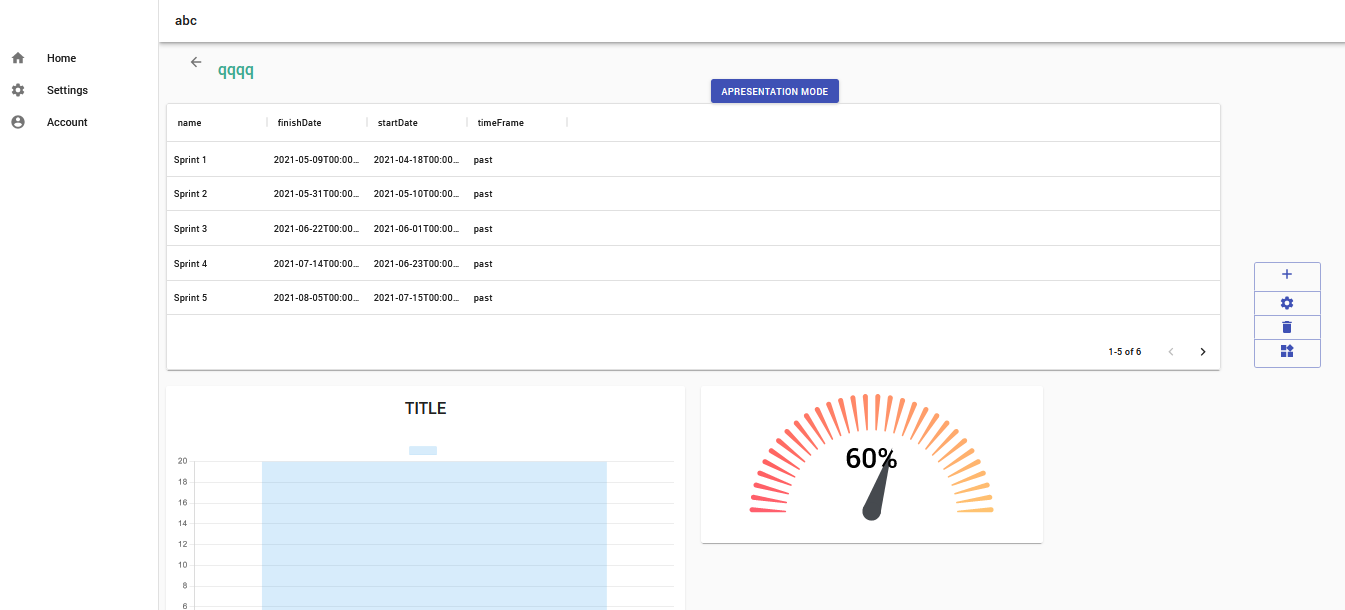
\includegraphics[width=\textwidth]{dashboardPage.png}
\caption{Dashboard Page and Widget View}
\end{figure}

\section{Settings Page}
This view is where the user can change the application's display language. If the user is a superuser, he can add users to the Lean Dashboard application or access the User Management page where all the users in the application can be viewed and edited, by adding or deleting roles for a specific user, deleting users, or changing his username or password. 

\begin{figure}[h!]
\center
  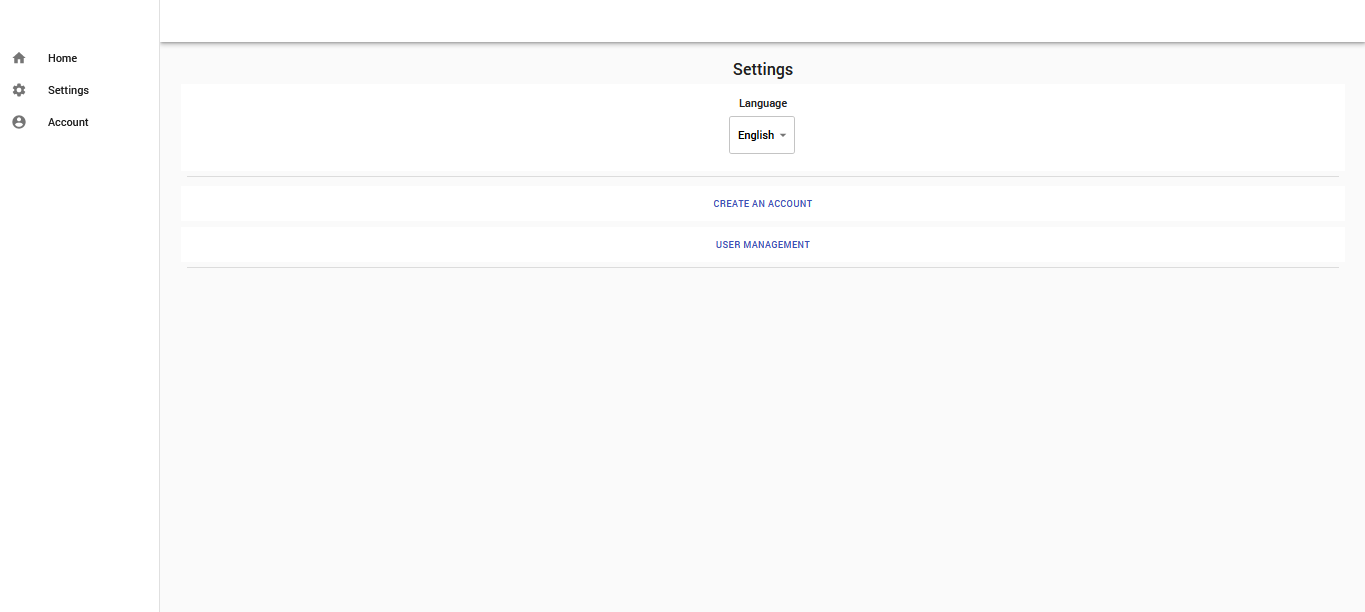
\includegraphics[width=\textwidth]{settingsPage.png}
\caption{Settings Page}
\end{figure}
\section{User Management}
The application needed an interface to manage the users and their roles. The view is a table or list of all Lean Dashboard users, and the superuser can assign roles or remove them from a user. The superuser can either change the username or password of a user and delete his account.
\begin{figure}[h!]
\center
  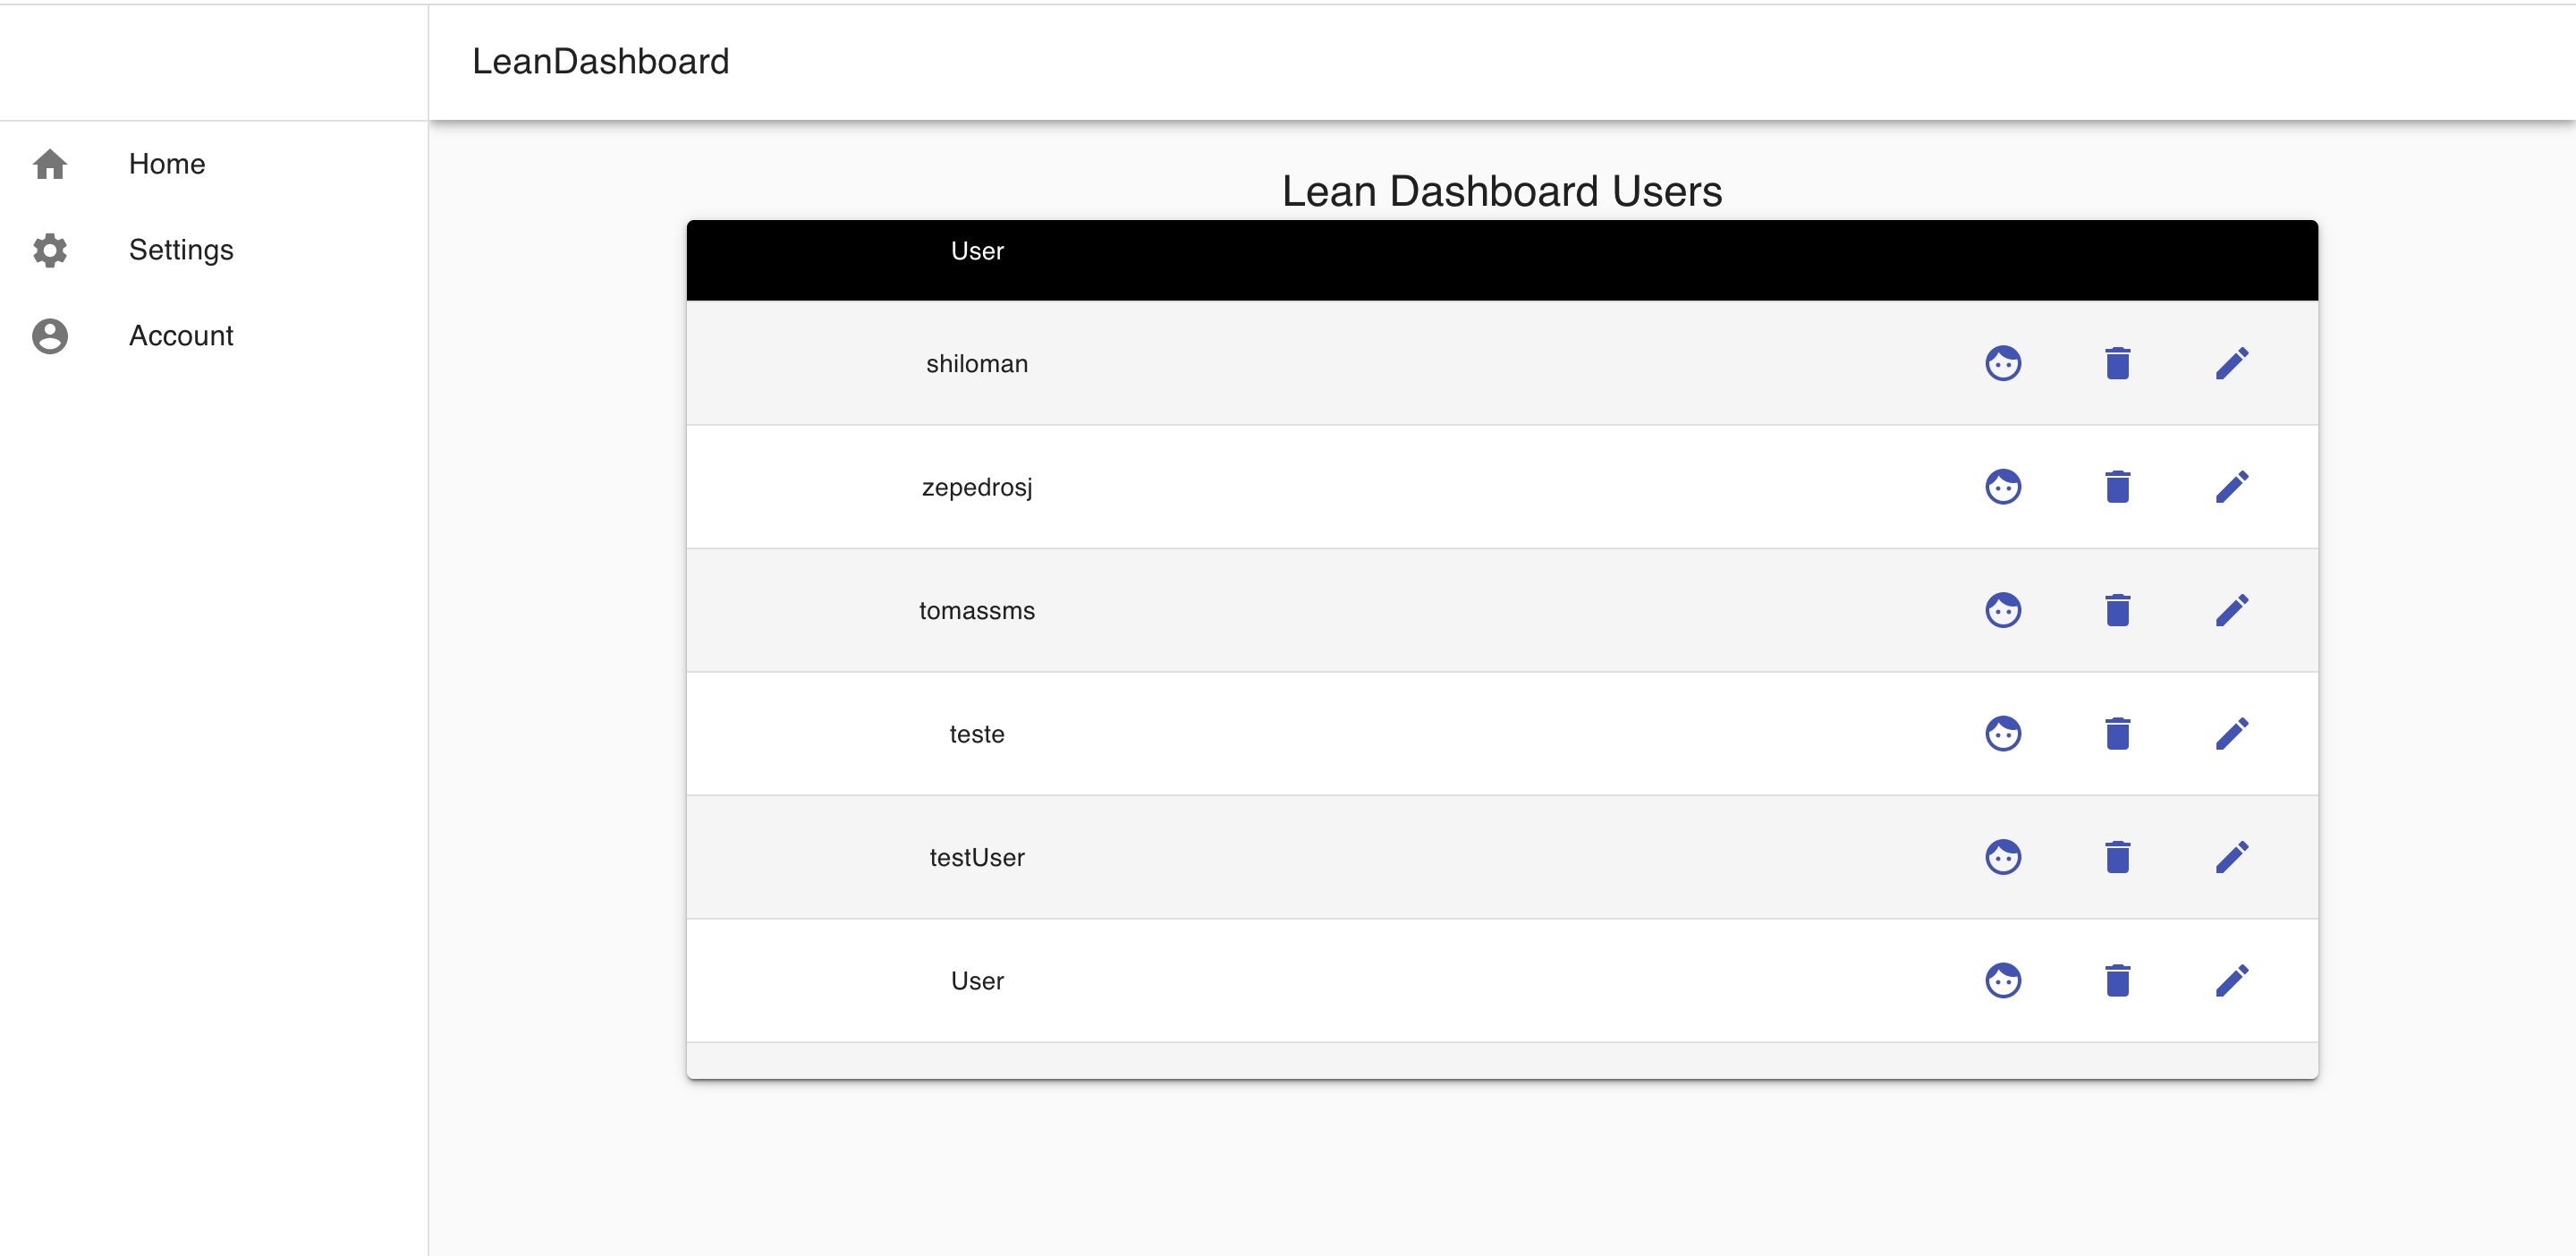
\includegraphics[width=\textwidth]{UserManagement.png}
\caption{User Management}
\end{figure}
\section{Projects Settings}
All the project settings are dealt with on this page, where the project manager or superuser can change the name or description of the projects, add users or platform credentials, that will later be used to add widgets.

\begin{figure}[h!]
\center
  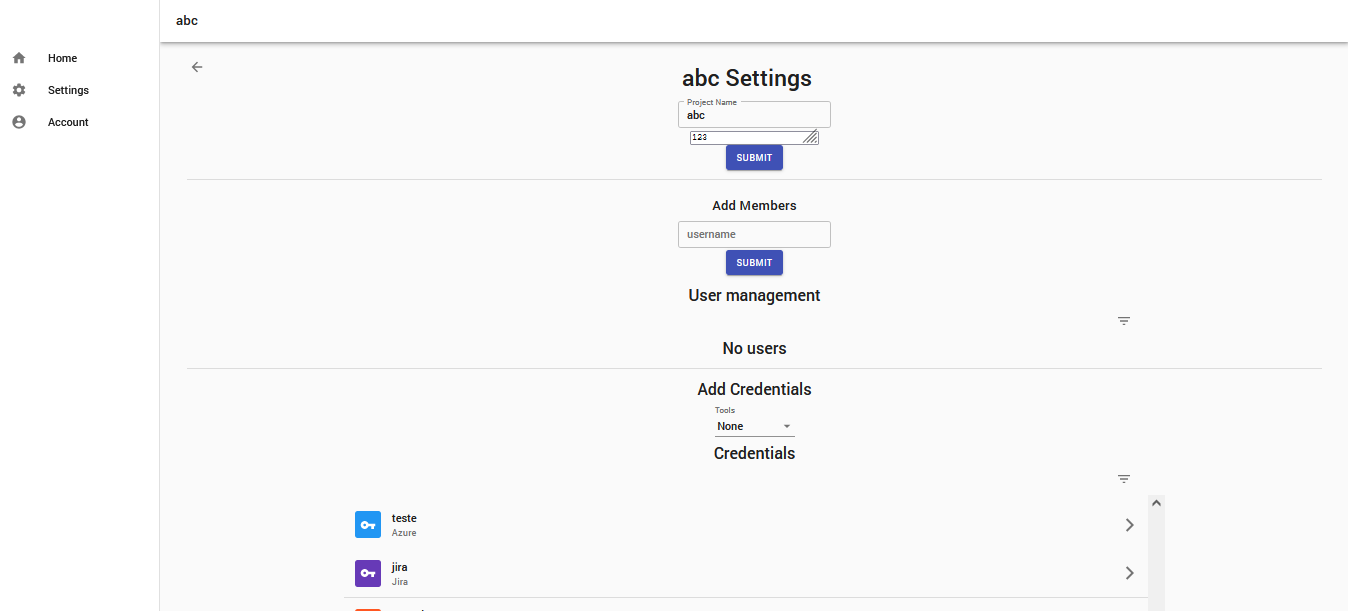
\includegraphics[width=\textwidth]{projectsettingsPage.png}
\caption{Project Settings Page}
\end{figure}

\chapter{Work Methodology and Deployment}
This chapter explained the methodology and what the team did to ensure the quality of work in this application and deployment. 

\section{Tests}

To guarantee the server's robustness, the team made numerous tests. The analysis was the possible error situations and their results and the successful cases. The technology that chooses to do the tests was Frisby.

\begin{figure}[h!]
\center
  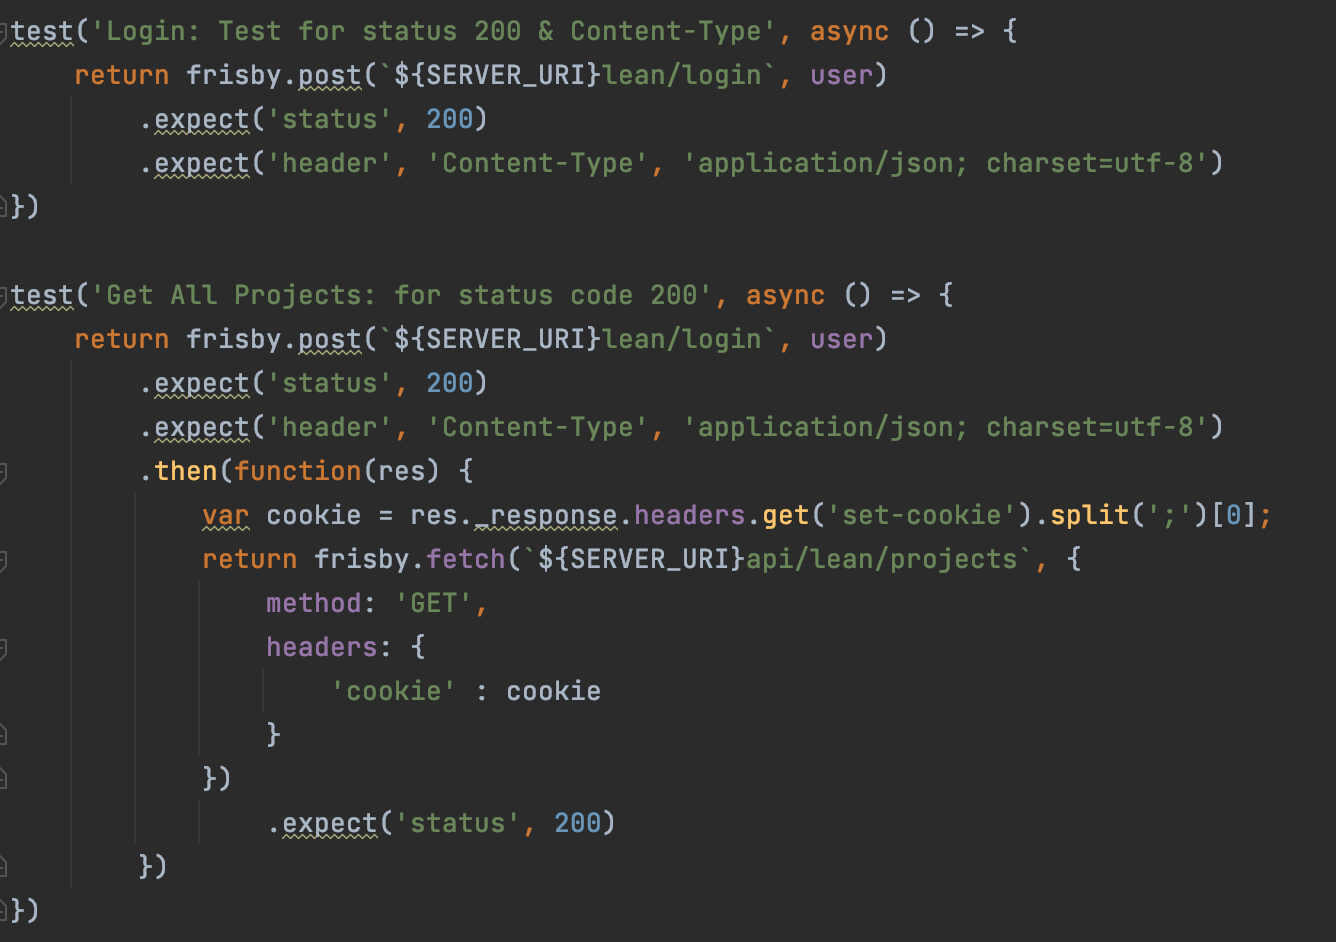
\includegraphics[width=\textwidth]{tests.png}
\caption{Unit test implementation example}
\end{figure}

The figure above illustrates two unit tests, the first one is a successful login and the second is to get all project belongs to the superuser.

\section{Deployment}
For the deployment of the application, we ended up choosing the Heroku\cite{HEROKU} platform. This was the platform chosen since it was used previously in the Software Laboratory course and thus all three students add some experience with the procedure of deploying an application on this service.

To take care of the storage of all the users and the projects (and their respective dashboards and widgets) we used two addons: Heroku Postgres\cite{HEROKUPOSTGRES} and Bonsai Elasticsearch\cite{BONSAIELASTICSEARCH}, respectively.

After having the storage situation handled, we followed the official React guide for deploying an application\cite{REACTDEPLOYMENT}. With that, we then followed the guide from the Heroku Buildpack for Create React App, with a Node.js server
\chapter{Conclusion}

Developing this project, allowed the team to apply the experience acquired along the course in this project.

This project provided the opportunity to work with Inetum and developing a web application, from back to front, as well as interacting with other applications in order to learn how to implement the necessary API requests to obtain the ETL data.

The project also taught the group a lot about the research and planning of an application's user experience as the team has never been introduced to such a topic. Conducting the research on UX and usability tests showed us a new perspective on application development.

In the long term, the following versions can have other functionalities like features to the digital accessibility, which means making the application more inclusive for all users, drag and drop the widgets in the dashboard making the dashboard more configurable, and creation of more widgets.

According to our initial planning, some of the tasks took longer than we were expecting, especially the ETL procedure as it took some time to learn and adapt to our application, but overall the application was finished successfully with good results solving the main problem of aggregating all the spread information in one place for a team to see while having an easy to use and intuitive design that adapts to every type of device and supports various display languages.





\begin{thebibliography} {websites}

\bibitem{INETUM} Inetum https://gfi.world/pt-en/

\bibitem{JIRA} Jira- Software development tool used by agile teams
https://www.atlassian.com/software/jira

\bibitem{SQUASH} Squash - Suite tool for test management
https://www.squashtest.com/?lang=en

\bibitem{AZURE} Azure - Cloud computing service by Microsoft
https://azure.microsoft.com/en-us/

\bibitem{RBAC} RBAC - Role-based Access Control
\texttt{https://en.wikipedia.org/wiki/Role-based\_access\_control}

\bibitem{INFOARCH} Information Architecture
\texttt{https://en.wikipedia.org/wiki/Information\_architecture}

\bibitem{REACT} React https://reactjs.org/

\bibitem{ETLPROC} ETL - Understanding It and Effectively Using It.
https://medium.com/hashmapinc/etl-understanding-it-and-effectively-using-it-f827a5b3e54d
Consulted on April 1st, 2021

\bibitem{AUTHIZATION} Authization Module
https://github.com/dleandro/Authentication-and-Authorization-Node-Component-

\bibitem{POSTGRESQL} PostgreSQL: The World's Most Advanced Open Source Relational Database
https://www.postgresql.org/

\bibitem{MIRO} Miro - Platform used for the Information Architecture schema
https://miro.com/

\bibitem{FIGMA} Figma Prototype toolhttps://www.figma.com/prototyping/

\bibitem{ES} ElasticSearch https://www.elastic.co/elasticsearch/

\bibitem{NODE} Node.JS https://nodejs.org/en/

\bibitem{NODECRON} node-cron https://www.npmjs.com/package/node-cron

\bibitem{USESTATE} Using the State Hook
https://reactjs.org/docs/hooks-state.html

\bibitem{USEEFFECT} Using the Effect Hook
https://reactjs.org/docs/hooks-effect.html

\bibitem{USECONTEXT} Context Hook
https://reactjs.org/docs/context.html

\bibitem{USEFETCH} Fetch Hook
https://use-http.com

\bibitem{HEROKU} Heroku - Cloud Application Platform
https://www.heroku.com/home

\bibitem{HEROKUPOSTGRES} - Heroku Postgres
https://www.heroku.com/postgres

\bibitem{BONSAIELASTICSEARCH} - Bonsai Elasticsearch
https://bonsai.io/

\bibitem{REACTDEPLOYMENT} - React Deployment
https://create-react-app.dev/docs/deployment/
\end{thebibliography}



\appendix

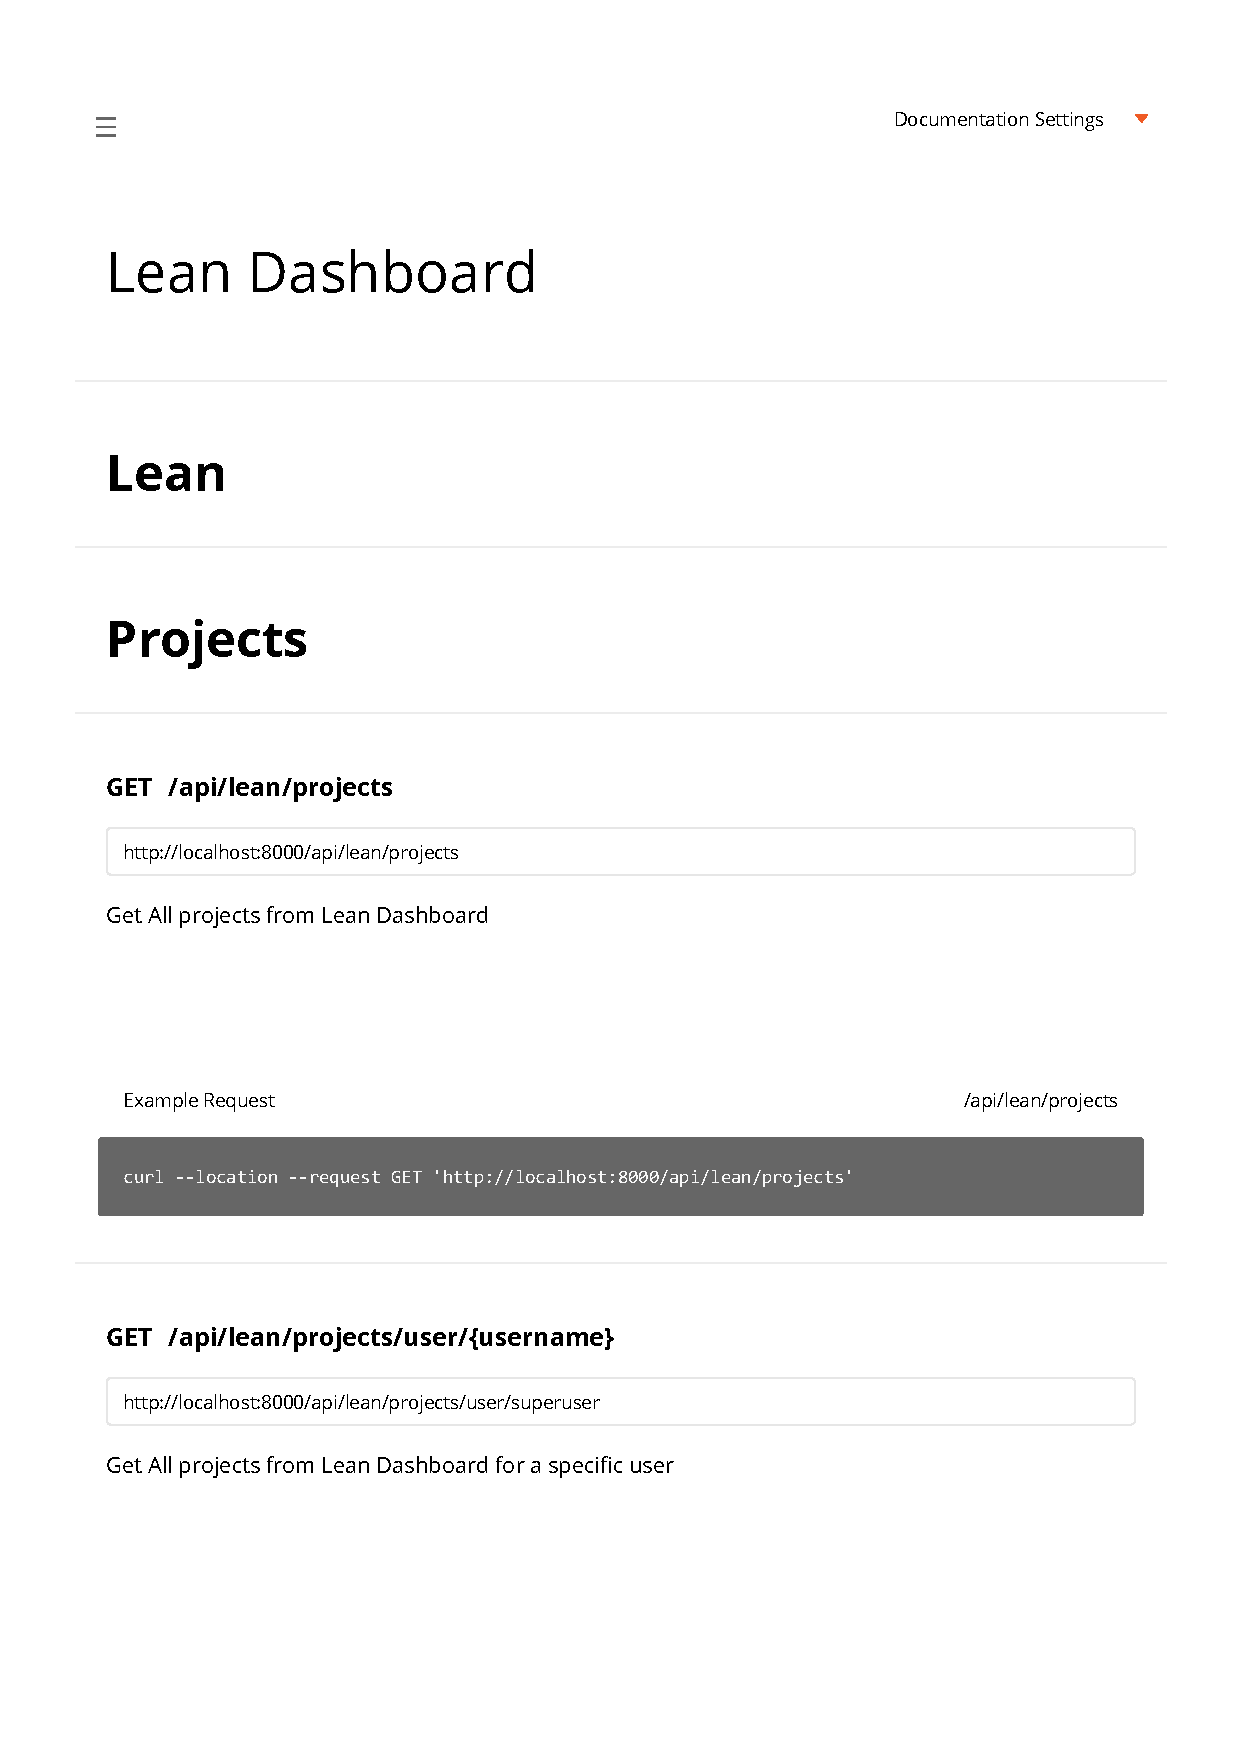
\includepdf[pages=1,scale=0.9,offset=0mm -75,pagecommand={
 \begin{flushleft}  
  \section*{Appendix A - API Documentation}
 \end{flushleft}}]{API Documentation.pdf}

\includepdf[pages=2-,scale=0.9]{API Documentation.pdf}

\end{document}

